
\documentclass[12pt,a4paper, oneside]{extreport}

%%%%%%%%%% Математика %%%%%%%%%%
\usepackage{amsmath,amsfonts,amssymb,amsthm,mathtools}
% Показывать номера только у тех формул, на которые есть \eqref{} в тексте.
%\mathtoolsset{showonlyrefs=true}
%\usepackage{leqno} % Нумерация формул слева
%\usepackage{tipa} %Для формулки из логитов


\usepackage{hyphenat}

%%%%%%%%%% Шрифты %%%%%%%%
\usepackage[english, russian]{babel} % выбор языка для документа
\usepackage[utf8]{inputenc} % задание utf8 кодировки исходного tex файла
\usepackage[X2,T2A]{fontenc}        % кодировка

\usepackage{fontspec}         % пакет для подгрузки шрифтов
\setmainfont{Times New Roman}       % задаёт основной шрифт документа

\usepackage{unicode-math}      % пакет для установки математического шрифта
\setmathfont{Asana-Math.otf}    % шрифт для математики

% Конкретный символ из конкретного шрифта
% \setmathfont[range=\int]{Neo Euler}


%%%%%%%%%% Работа с картинками %%%%%%%%%
\usepackage{graphicx}                  % Для вставки рисунков
\usepackage{graphics}
\graphicspath{{images/}{pictures/}}    % можно указать папки с картинками
\usepackage{wrapfig}                   % Обтекание рисунков и таблиц текстом


%%%%%%%%%% Работа с таблицами %%%%%%%%%%
\usepackage{tabularx}            % новые типы колонок
\usepackage{tabulary}            % и ещё новые типы колонок
\usepackage{array,delarray}      % Дополнительная работа с таблицами
\usepackage{longtable}           % Длинные таблицы
\usepackage{multirow}            % Слияние строк в таблице
\usepackage{float}               % возможность позиционировать объекты в нужном месте

\usepackage{booktabs}            % таблицы как в книгах

% Заповеди из документации к booktabs:
% 1. Будь проще! Глазам должно быть комфортно
% 2. Не используйте вертикальные линни
% 3. Не используйте двойные линии. Как правило, достаточно трёх горизонтальных линий
% 4. Единицы измерения - в шапку таблицы
% 5. Не сокращайте .1 вместо 0.1
% 6. Повторяющееся значение повторяйте, а не говорите "то же"
% 7. Есть сомнения? Выравнивай по левому краю!

%  вычисляемые колонки по tabularx
\newcolumntype{C}{>{\centering\arraybackslash}X}
\newcolumntype{L}{>{\raggedright\arraybackslash}X}
\newcolumntype{Y}{>{\arraybackslash}X}
\newcolumntype{Z}{>{\centering\arraybackslash}X}


%%%%%%%%%% Графика и рисование %%%%%%%%%%
\usepackage{tikz, pgfplots}      % язык для рисования графики из latex'a

%%%%%%%%%% Гиперссылки %%%%%%%%%%
\usepackage{xcolor}              % разные цвета

\usepackage{hyperref}
\hypersetup{
	unicode=true,           % позволяет использовать юникодные символы
	colorlinks=true,       	% true - цветные ссылки, false - ссылки в рамках
	urlcolor =blue,         % цвет ссылки на url
	linkcolor=black,        % внутренние ссылки
	citecolor=black,        % на библиографию
	breaklinks              % если ссылка не умещается в одну строку, разбивать ли ее на две части?
}


%%%%%%%%%% Другие приятные пакеты %%%%%%%%%
\usepackage{multicol}       % несколько колонок
\usepackage{verbatim}       % для многострочных комментариев
\usepackage{cmap} % для кодировки шрифтов в pdf

\usepackage{enumitem} % дополнительные плюшки для списков
%  например \begin{enumerate}[resume] позволяет продолжить нумерацию в новом списке

\usepackage{todonotes} % для вставки в документ заметок о том, что  осталось сделать
% \todo{Здесь надо коэффициенты исправить}
% \missingfigure{Здесь будет Последний день Помпеи}
% \listoftodos --- печатает все поставленные \todo'шки



%%%%%%%%%%%%%% ГОСТОВСКИЕ ПРИБАМБАСЫ %%%%%%%%%%%%%%%

%%% размер листа бумаги
\usepackage[paper=a4paper,top=15mm, bottom=15mm,left=35mm,right=10mm,includehead]{geometry}


\usepackage{setspace}
\setstretch{1.5}     % Межстрочный интервал
\setlength{\parindent}{1.63em} % Красная строка.


%\flushbottom       % Эта команда заставляет LaTeX чуть растягивать строки, чтобы получить идеально прямоугольную страницу
\righthyphenmin=2  % Разрешение переноса двух и более символов
\widowpenalty=10000  % Наказание за вдовствующую строку (одна строка абзаца на этой странице, остальное --- на следующей)
\clubpenalty=10000  % Наказание за сиротствующую строку (омерзительно висящая одинокая строка в начале страницы)
\tolerance=1000     % Ещё какое-то наказание.


% Нумерация страниц сверху по центру
\usepackage{fancyhdr}
\pagestyle{fancy}
\fancyhead{ } % clear all fields
\fancyfoot{ } % clear all fields
\fancyhead[C]{\thepage}
% Чтобы не прорисовывалась черта!
\renewcommand{\headrulewidth}{0pt}


% Нумерация страниц с надписью "Глава"
\usepackage{etoolbox}
\patchcmd{\chapter}{\thispagestyle{plain}}{\thispagestyle{fancy}}{}{}


%%% Заголовки
\usepackage[indentfirst]{titlesec}{\raggedleft}
% Заголовки по левому краю
% опция identfirst устанавливает отступ в первом абзаце


% Редактирования Глав и названий
\titleformat{\chapter}
{\normalfont\large\bfseries}
{\thechapter }{0.5 em}{}

% Редактирование ненумеруемых глав chapter* (Введение и тп)
\titleformat{name=\chapter,numberless}
{\centering\normalfont\bfseries\large}{}{0.25em}{\normalfont}

% Убирает чеканутые отступы вверху страницы
\titlespacing{\chapter}{0pt}{-\baselineskip}{\baselineskip}

% Более низкие уровни
\titleformat{\section}{\bfseries}{\thesection}{0.5 em}{}
\titleformat{\subsection}{\bfseries}{\thesubsection}{0.5 em}{}

\titlespacing*{\section}{0 pt}{\baselineskip}{\baselineskip}
\titlespacing*{\subsection}{0 pt}{\baselineskip}{\baselineskip}


% Содержание. Команды ниже изменяют отступы и рисуют точечки!
\usepackage{titletoc}

\titlecontents{chapter}
[1em] %
{\normalsize}
{\contentslabel{1 em}}
{\hspace{-1 em}}
{\normalsize\titlerule*[10pt]{.}\contentspage}

\titlecontents{section}
[3 em] %
{\normalsize}
{\contentslabel{1.75 em}}
{\hspace{-1.75 em}}
{\normalsize\titlerule*[10pt]{.}\contentspage}

\titlecontents{subsection}
[6 em] %
{\normalsize}
{\contentslabel{3 em}}
{\hspace{-3 em}}
{\normalsize\titlerule*[10pt]{.}\contentspage}


% Правильные подписи под таблицей и рисунком
% Документация к пакету на русском языке!
\usepackage[tableposition=top, singlelinecheck=false]{caption}
\usepackage{subcaption}


\DeclareCaptionStyle{base}%
[justification=centering,indention=0pt]{}
\DeclareCaptionLabelFormat{gostfigure}{Рисунок #2}
\DeclareCaptionLabelFormat{gosttable}{Таблица #2}

\DeclareCaptionLabelSeparator{gost}{~---~}
\captionsetup{labelsep=gost}

\DeclareCaptionStyle{fig01}%
[margin=5mm,justification=centering]%
{margin={3em,3em}}
\captionsetup*[figure]{style=fig01,labelsep=gost,labelformat=gostfigure,format=hang}

\DeclareCaptionStyle{tab01}%
[margin=5mm,justification=centering]%
{margin={3em,3em}}
\captionsetup*[table]{style=tab01,labelsep=gost,labelformat=gosttable,format=hang}


% межстрочный отступ в таблице
\renewcommand{\arraystretch}{1.2}



% многостраничные таблицы под РОССИЙСКИЙ СТАНДАРТ
% ВНИМАНИЕ! Обязательно за CAPTION !
\usepackage{fr-longtable}



%Более гибкие спсики
\usepackage{enumitem}
% сообщаем окружению о том, что существует такая штук как нумерация русскими буквами.
\makeatletter
\AddEnumerateCounter{\asbuk}{\russian@alph}{щ}
\makeatother


%%% ГОСТОВСКИЕ СПИСКИ

% Первый тип списков. Большая буква.
\newlist{Enumerate}{enumerate}{1}

\setlist[Enumerate,1]{labelsep=0.5em,leftmargin=1.25em,labelwidth=1.25em,
	parsep=0em,itemsep=0em,topsep=0ex, before={\parskip=-1em},label=\arabic{Enumeratei}.}


% Второй тип списков. Маленькая буква.
\setlist[enumerate]{label=\arabic{enumi}),parsep=0em,itemsep=0em,topsep=0.75ex, before={\parskip=-1em}}


% Третий тип списков. Два уровня.
\newlist{twoenumerate}{enumerate}{2}
\setlist[twoenumerate,1]{itemsep=0mm,parsep=0em,topsep=0.75ex,, before={\parskip=-1em},label=\asbuk{twoenumeratei})}
\setlist[twoenumerate,2]{leftmargin=1.3em,itemsep=0mm,parsep=0em,topsep=0ex, before={\parskip=-1em},label=\arabic{twoenumerateii})}


% Четвёртый тип списков. Список с тире.
\setlist[itemize]{label=--,parsep=0em,itemsep=0em,topsep=0ex, before={\parskip=-1em},after={\parskip=-1em}}


%%% WARNING WARNING WARNIN!
%%% Если в списке предложения, то должна по госту стоять точка после цифры => команда Enumerate! Если идет перечень маленьких фактов, не обособляемых предложений то после цифры идет скобка ")" => команда enumerate! Если перечень при этом ещё и двууровневый, то twoenumerate.




%%%%%%%%%% Список литературы %%%%%%%%%%

%\usepackage[%
%backend=biber, %подключение пакета biber (тоже нужен)
%bibstyle=gost-numeric, %подключение одного из четырех главных стилей biblatex-gost
%sorting=ntvy, %тип сортировки в библиографии
%]{biblatex}

\usepackage[backend=biber,style=gost-numeric, maxbibnames=9,maxcitenames=2,uniquelist=false, babel=other]{biblatex}



% Справка по 4 главным стилям для ленивых:
% gost-inline  ссылки внутри теста в круглых скобках
% gost-footnote подстрочные ссылки
% gost-numeric затекстовые ссылки
% gost-authoryear тоже затекстовые ссылки, но немного другие

% Подробнее смотри страницу 4 документации. Она на русском.

% Ещё немного настроек
\DeclareFieldFormat{postnote}{#1} %убирает с. и p.
\renewcommand*{\mkgostheading}[1]{#1} % только лишь убираем курсив с авторов


\addbibresource{bib.bib} % сюда нужно вписать свой bib-файлик.


%\usepackage{appendix}


% Этот кусок кода выносит русские источники на первое место. Костыль описали авторы пакета в руководстве к нему. Подробнее смотри:
% https://github.com/odomanov/biblatex-gost/wiki/Как-сделать%2C-чтобы-русскоязычные-источники-предшествовали-остальным
\DeclareSourcemap{
	\maps[datatype=bibtex]{
		\map{
			\step[fieldsource=langid, match=russian, final]
			\step[fieldset=presort, fieldvalue={a}]
		}
		\map{
			\step[fieldsource=langid, notmatch=russian, final]
			\step[fieldset=presort, fieldvalue={z}]
		}
	}
}

\DefineBibliographyStrings{english}{%
	pages = {P\adddot},
	number = {№},
}

\documentclass[12pt,a4paper, oneside]{extreport}

%%%%%%%%%% Математика %%%%%%%%%%
\usepackage{amsmath,amsfonts,amssymb,amsthm,mathtools}
% Показывать номера только у тех формул, на которые есть \eqref{} в тексте.
%\mathtoolsset{showonlyrefs=true}
%\usepackage{leqno} % Нумерация формул слева
%\usepackage{tipa} %Для формулки из логитов


\usepackage{hyphenat}

%%%%%%%%%% Шрифты %%%%%%%%
\usepackage[english, russian]{babel} % выбор языка для документа
\usepackage[utf8]{inputenc} % задание utf8 кодировки исходного tex файла
\usepackage[X2,T2A]{fontenc}        % кодировка

\usepackage{fontspec}         % пакет для подгрузки шрифтов
\setmainfont{Times New Roman}       % задаёт основной шрифт документа

\usepackage{unicode-math}      % пакет для установки математического шрифта
\setmathfont{Asana-Math.otf}    % шрифт для математики

% Конкретный символ из конкретного шрифта
% \setmathfont[range=\int]{Neo Euler}


%%%%%%%%%% Работа с картинками %%%%%%%%%
\usepackage{graphicx}                  % Для вставки рисунков
\usepackage{graphics}
\graphicspath{{images/}{pictures/}}    % можно указать папки с картинками
\usepackage{wrapfig}                   % Обтекание рисунков и таблиц текстом


%%%%%%%%%% Работа с таблицами %%%%%%%%%%
\usepackage{tabularx}            % новые типы колонок
\usepackage{tabulary}            % и ещё новые типы колонок
\usepackage{array,delarray}      % Дополнительная работа с таблицами
\usepackage{longtable}           % Длинные таблицы
\usepackage{multirow}            % Слияние строк в таблице
\usepackage{float}               % возможность позиционировать объекты в нужном месте

\usepackage{booktabs}            % таблицы как в книгах

% Заповеди из документации к booktabs:
% 1. Будь проще! Глазам должно быть комфортно
% 2. Не используйте вертикальные линни
% 3. Не используйте двойные линии. Как правило, достаточно трёх горизонтальных линий
% 4. Единицы измерения - в шапку таблицы
% 5. Не сокращайте .1 вместо 0.1
% 6. Повторяющееся значение повторяйте, а не говорите "то же"
% 7. Есть сомнения? Выравнивай по левому краю!

%  вычисляемые колонки по tabularx
\newcolumntype{C}{>{\centering\arraybackslash}X}
\newcolumntype{L}{>{\raggedright\arraybackslash}X}
\newcolumntype{Y}{>{\arraybackslash}X}
\newcolumntype{Z}{>{\centering\arraybackslash}X}


%%%%%%%%%% Графика и рисование %%%%%%%%%%
\usepackage{tikz, pgfplots}      % язык для рисования графики из latex'a

%%%%%%%%%% Гиперссылки %%%%%%%%%%
\usepackage{xcolor}              % разные цвета

\usepackage{hyperref}
\hypersetup{
	unicode=true,           % позволяет использовать юникодные символы
	colorlinks=true,       	% true - цветные ссылки, false - ссылки в рамках
	urlcolor =blue,         % цвет ссылки на url
	linkcolor=black,        % внутренние ссылки
	citecolor=black,        % на библиографию
	breaklinks              % если ссылка не умещается в одну строку, разбивать ли ее на две части?
}


%%%%%%%%%% Другие приятные пакеты %%%%%%%%%
\usepackage{multicol}       % несколько колонок
\usepackage{verbatim}       % для многострочных комментариев
\usepackage{cmap} % для кодировки шрифтов в pdf

\usepackage{enumitem} % дополнительные плюшки для списков
%  например \begin{enumerate}[resume] позволяет продолжить нумерацию в новом списке

\usepackage{todonotes} % для вставки в документ заметок о том, что  осталось сделать
% \todo{Здесь надо коэффициенты исправить}
% \missingfigure{Здесь будет Последний день Помпеи}
% \listoftodos --- печатает все поставленные \todo'шки



%%%%%%%%%%%%%% ГОСТОВСКИЕ ПРИБАМБАСЫ %%%%%%%%%%%%%%%

%%% размер листа бумаги
\usepackage[paper=a4paper,top=15mm, bottom=15mm,left=35mm,right=10mm,includehead]{geometry}


\usepackage{setspace}
\setstretch{1.5}     % Межстрочный интервал
\setlength{\parindent}{1.63em} % Красная строка.


%\flushbottom       % Эта команда заставляет LaTeX чуть растягивать строки, чтобы получить идеально прямоугольную страницу
\righthyphenmin=2  % Разрешение переноса двух и более символов
\widowpenalty=10000  % Наказание за вдовствующую строку (одна строка абзаца на этой странице, остальное --- на следующей)
\clubpenalty=10000  % Наказание за сиротствующую строку (омерзительно висящая одинокая строка в начале страницы)
\tolerance=1000     % Ещё какое-то наказание.


% Нумерация страниц сверху по центру
\usepackage{fancyhdr}
\pagestyle{fancy}
\fancyhead{ } % clear all fields
\fancyfoot{ } % clear all fields
\fancyhead[C]{\thepage}
% Чтобы не прорисовывалась черта!
\renewcommand{\headrulewidth}{0pt}


% Нумерация страниц с надписью "Глава"
\usepackage{etoolbox}
\patchcmd{\chapter}{\thispagestyle{plain}}{\thispagestyle{fancy}}{}{}


%%% Заголовки
\usepackage[indentfirst]{titlesec}{\raggedleft}
% Заголовки по левому краю
% опция identfirst устанавливает отступ в первом абзаце


% Редактирования Глав и названий
\titleformat{\chapter}
{\normalfont\large\bfseries}
{\thechapter }{0.5 em}{}

% Редактирование ненумеруемых глав chapter* (Введение и тп)
\titleformat{name=\chapter,numberless}
{\centering\normalfont\bfseries\large}{}{0.25em}{\normalfont}

% Убирает чеканутые отступы вверху страницы
\titlespacing{\chapter}{0pt}{-\baselineskip}{\baselineskip}

% Более низкие уровни
\titleformat{\section}{\bfseries}{\thesection}{0.5 em}{}
\titleformat{\subsection}{\bfseries}{\thesubsection}{0.5 em}{}

\titlespacing*{\section}{0 pt}{\baselineskip}{\baselineskip}
\titlespacing*{\subsection}{0 pt}{\baselineskip}{\baselineskip}


% Содержание. Команды ниже изменяют отступы и рисуют точечки!
\usepackage{titletoc}

\titlecontents{chapter}
[1em] %
{\normalsize}
{\contentslabel{1 em}}
{\hspace{-1 em}}
{\normalsize\titlerule*[10pt]{.}\contentspage}

\titlecontents{section}
[3 em] %
{\normalsize}
{\contentslabel{1.75 em}}
{\hspace{-1.75 em}}
{\normalsize\titlerule*[10pt]{.}\contentspage}

\titlecontents{subsection}
[6 em] %
{\normalsize}
{\contentslabel{3 em}}
{\hspace{-3 em}}
{\normalsize\titlerule*[10pt]{.}\contentspage}


% Правильные подписи под таблицей и рисунком
% Документация к пакету на русском языке!
\usepackage[tableposition=top, singlelinecheck=false]{caption}
\usepackage{subcaption}


\DeclareCaptionStyle{base}%
[justification=centering,indention=0pt]{}
\DeclareCaptionLabelFormat{gostfigure}{Рисунок #2}
\DeclareCaptionLabelFormat{gosttable}{Таблица #2}

\DeclareCaptionLabelSeparator{gost}{~---~}
\captionsetup{labelsep=gost}

\DeclareCaptionStyle{fig01}%
[margin=5mm,justification=centering]%
{margin={3em,3em}}
\captionsetup*[figure]{style=fig01,labelsep=gost,labelformat=gostfigure,format=hang}

\DeclareCaptionStyle{tab01}%
[margin=5mm,justification=centering]%
{margin={3em,3em}}
\captionsetup*[table]{style=tab01,labelsep=gost,labelformat=gosttable,format=hang}


% межстрочный отступ в таблице
\renewcommand{\arraystretch}{1.2}



% многостраничные таблицы под РОССИЙСКИЙ СТАНДАРТ
% ВНИМАНИЕ! Обязательно за CAPTION !
\usepackage{fr-longtable}



%Более гибкие спсики
\usepackage{enumitem}
% сообщаем окружению о том, что существует такая штук как нумерация русскими буквами.
\makeatletter
\AddEnumerateCounter{\asbuk}{\russian@alph}{щ}
\makeatother


%%% ГОСТОВСКИЕ СПИСКИ

% Первый тип списков. Большая буква.
\newlist{Enumerate}{enumerate}{1}

\setlist[Enumerate,1]{labelsep=0.5em,leftmargin=1.25em,labelwidth=1.25em,
	parsep=0em,itemsep=0em,topsep=0ex, before={\parskip=-1em},label=\arabic{Enumeratei}.}


% Второй тип списков. Маленькая буква.
\setlist[enumerate]{label=\arabic{enumi}),parsep=0em,itemsep=0em,topsep=0.75ex, before={\parskip=-1em}}


% Третий тип списков. Два уровня.
\newlist{twoenumerate}{enumerate}{2}
\setlist[twoenumerate,1]{itemsep=0mm,parsep=0em,topsep=0.75ex,, before={\parskip=-1em},label=\asbuk{twoenumeratei})}
\setlist[twoenumerate,2]{leftmargin=1.3em,itemsep=0mm,parsep=0em,topsep=0ex, before={\parskip=-1em},label=\arabic{twoenumerateii})}


% Четвёртый тип списков. Список с тире.
\setlist[itemize]{label=--,parsep=0em,itemsep=0em,topsep=0ex, before={\parskip=-1em},after={\parskip=-1em}}


%%% WARNING WARNING WARNIN!
%%% Если в списке предложения, то должна по госту стоять точка после цифры => команда Enumerate! Если идет перечень маленьких фактов, не обособляемых предложений то после цифры идет скобка ")" => команда enumerate! Если перечень при этом ещё и двууровневый, то twoenumerate.




%%%%%%%%%% Список литературы %%%%%%%%%%

%\usepackage[%
%backend=biber, %подключение пакета biber (тоже нужен)
%bibstyle=gost-numeric, %подключение одного из четырех главных стилей biblatex-gost
%sorting=ntvy, %тип сортировки в библиографии
%]{biblatex}

\usepackage[backend=biber,style=gost-numeric, maxbibnames=9,maxcitenames=2,uniquelist=false, babel=other]{biblatex}



% Справка по 4 главным стилям для ленивых:
% gost-inline  ссылки внутри теста в круглых скобках
% gost-footnote подстрочные ссылки
% gost-numeric затекстовые ссылки
% gost-authoryear тоже затекстовые ссылки, но немного другие

% Подробнее смотри страницу 4 документации. Она на русском.

% Ещё немного настроек
\DeclareFieldFormat{postnote}{#1} %убирает с. и p.
\renewcommand*{\mkgostheading}[1]{#1} % только лишь убираем курсив с авторов



% Этот кусок кода выносит русские источники на первое место. Костыль описали авторы пакета в руководстве к нему. Подробнее смотри:
% https://github.com/odomanov/biblatex-gost/wiki/Как-сделать%2C-чтобы-русскоязычные-источники-предшествовали-остальным
\DeclareSourcemap{
	\maps[datatype=bibtex]{
		\map{
			\step[fieldsource=langid, match=russian, final]
			\step[fieldset=presort, fieldvalue={a}]
		}
		\map{
			\step[fieldsource=langid, notmatch=russian, final]
			\step[fieldset=presort, fieldvalue={z}]
		}
	}
}

\DefineBibliographyStrings{english}{%
	pages = {P\adddot},
	number = {№},
}



\begin{document}
\thispagestyle{empty} % Чтобы избежать нумерации титульника

% !TEX root = ../main_file.tex

\thispagestyle{empty} % Чтобы избежать нумерации титульника

% Если для какой-то страницы хочется сделать своё уникальное оформление, как например для титульника или списка литературы, то можно использовать окружение \begingroup ... \endgroup. 

\begingroup
\setstretch{1} 
\begin{center}
\small \bfseries Федеральное государственное бюджетное образовательное учреждение высшего образования

«РОССИЙСКАЯ АКАДЕМИЯ НАРОДНОГО ХОЗЯЙСТВА и\\ ГОСУДАРСТВЕННОЙ СЛУЖБЫ \\
при Президенте Российской Федерации»

\vspace{2ex}

\bfseries
ИНСТИТУТ ЭКОНОМИКИ, МАТЕМАТИКИ И ИНФОРМАЦИОННЫХ\\ ТЕХНОЛОГИЙ

ЭКОНОМИЧЕСКИЙ ФАКУЛЬТЕТ 

НАПРАВЛЕНИЕ 38.03.01 ЭКОНОМИКА
\end{center}

\vfill

\noindent Группа ЭО-15-01
\hfill
\parbox[t]{20em}{\centering 
Кафедра микроэкономики

\mbox{ }

\textbf{Допустить к защите}

заведующий кафедрой микроэкономики

\mbox{ }

\rule{8em}{0.5pt} М.И. Левин

\mbox{ }

«\rule{2em}{0.5pt}» \rule{5em}{0.5pt} 201\rule{1em}{0.5pt} г. }

\mbox{ }

\mbox{ }

\begin{center}\bfseries
ВЫПУСКНАЯ КВАЛИФИКАЦИОННАЯ РАБОТА

\mbox{ }

\large
ПРОГНОЗИРОВАНИЕ И ОЦЕНКА МАКРОЭКОНОМИЧЕСКИХ ЗАВИСИМОСТЕЙ ПРИ ПОМОЩИ
МЕТОДОВ СНИЖЕНИЯ РАЗМЕРНОСТИ В ДАННЫХ НА ПРИМЕРЕ ИНВЕСТИЦИЙ В РОССИИ
\end{center}

\vfill

\noindent\normalsize
студент-бакалавр

\noindent
Гареев Михаил Юрьевич
\hfill /\rule{6em}{0.5pt}/\rule{6em}{0.5pt}/

\hfill\makebox[13em]{\hfill\footnotesize (подпись) \hfill\hfill (дата) \hfill}

\noindent
научный руководитель выпускной \\
квалификационной работы

\noindent
к.э.н., Полбин Андрей Владимирович
\hfill /\rule{6em}{0.5pt}/\rule{6em}{0.5pt}/

\hfill\makebox[13em]{\hfill\footnotesize (подпись) \hfill\hfill (дата) \hfill}

%\noindent
%консультант
%
%\noindent
%д.э.н., профессор Петров Петр Петрович
%\hfill /\rule{6em}{0.5pt}/\rule{6em}{0.5pt}/
%
%\hfill\makebox[13em]{\hfill\footnotesize (подпись) \hfill\hfill (дата) \hfill}

\vfill

\begin{center}
\normalsize \bfseries МОСКВА \\ 2019 г.
\end{center}
\endgroup
\newpage
 \tableofcontents
 \newpage
 
 \chapter*{Введение} \addcontentsline{toc}{chapter}{\protect\numberline{Введение}}
 Прогнозирование инвестиций --- сложная и интересная задача. Потенциально инвестиции зависит от большого количества наблюдаемых и ненаблюдаемых факторов. Поскольку принципиально невозможно учесть все из них, зачастую для прогнозирования могут использоваться простые модели временных рядов, (например, модель акселератора, рассмотренная ниже, включает лишь один фактор), или же вовсе наивный прогноз. Данная работа освещает некоторые возможные методы прогнозирования инвестиций при помощи обширных данных макроэкономической статистики. Ключевая идея всех этих методов --- некоторый автоматический отбор объясняющих переменных из довольно большого списка, или иными словами, снижение размерности в данных.

 Структура работы следующая: в главе \ref{ch:lit} произведен обзор литературы по рассматриваемой теме. В главе \ref{ch:models} приведено описание моделей, которые тестируются в данной работе, а также мотивация их применения. Глава \ref{ch:data} содержит  описание использованных данных, способы их трансформации и методологию построения прогнозов. В главе \ref{ch:results} содержатся эмпирические результаты исследования и их интерпретация. Глава \ref{ch:final} завершает исследование.

 \chapter{Обзор литературы} \label{ch:lit}

 С ростом популярности машинного обучения в последние десятилетия появилось множество различных методов оценивания моделей с большим количеством переменных. Общая идея состоит в том, чтобы каким-то образом исключить  <<мусорные>> переменные или снизить их влияние на предсказанные значения. И, хотя первоначально они разрабатывались для несколько других целей, эти методы могут использоваться и в прогнозировании макроэкономических зависимостей, в т.ч. при прогнозировании инвестиций. Важно отметить несколько особенностей, которые затрудняют прогнозирование.
 \begin{enumerate}
     \item Во-первых, это потенциально высокий риск структурных сдвигов, затрудняющих прогнозы. Это происходит, в частности, из-за зависимости от политических факторов.
     \item Во-вторых, теоретические результаты могут влиять на будущие показатели (вообще говоря, это, конечно, общая проблема экономики, но нужно помнить, что т.н. критика Лукаса \cite{lucas1976econometric},
     обратившая внимание на эту проблему, относилась именно к макроэкономическим зависимостям).
 \end{enumerate}

 Помимо трудностей прогнозирования, возникающих из-за возможного и вероятного переобучения при использовании моделей с высокой размерностью в данных, можно говорить и о трудностях интерпретации, т.к. выбор значимых переменных ведётся автоматически и обычно не предполагает каких-то априорных знаний о зависимостях. С другой стороны, используемый в этой работе подход потенциально позволяет выявить ранее неизвестные и неожиданные закономерности и, возможно, натолкнет на теоретические обоснования этих закономерностей. Подкрепить эту точку зрения можно мнение одного из основателей эконометрики Тинбергена, который в т.н. <<споре о методе>> с Кейнсом (последний критиковал эконометристов за порой бездумный чересчур математических подход к экономике), защищая эконометрику, приводил в пример зависимость между реальной ставкой и спросом на деньги, которая должна была наблюдаться по теоретическим обоснования, но при этом наблюдалась в реальных данных по американской экономике в тот период довольно слабо, что могло говорить об ошибках теории.
 
 
 Обобщающей работой по методам регуляризации можно назвать работу \cite{belloni2011high}
 в которой описан метод LASSO и его практическое применение, в том числе и в макроэкономике. В частности, приводится пример использования LASSO для тестирования гипотезы о конвергенции на основе мировой макроэкономической статистики конца XX века.
 
 Кроме этого, в той же работе приводится обоснование для использования метода Post-LASSO, который рассмотрен ниже и кратко состоит в том что сначала исключаются ненужные переменные, а после этого модель оценивается при помощи обычной линейной регрессии. Post-LASSO теоретически позволяет получить менее смещенные оценки, чем обычный метод LASSO.
 
 Существует и другая модификация метода LASSO, рассмотренная в работе \cite{zou2006adaptive}.
 В этой работе показывается, что в некоторых ситуациях LASSO неверно выбирает переменные. Из-за этого предлагается другая версия LASSO --- адаптивный LASSO, в котором используются веса для штрафов коэффициентов. В этом случае при определенных предпосылках метод отбирает верные переменные, и, кроме того, можно говорить о состоятельности полученных таким образом оценок коэффициентов.
 
 
 Другой метод регуляризации, регрессия гребня (Ridge) был описан в работе \cite{hoerl1970ridge}. Отличительной особенностью этого метода является то, что коэффициенты не зануляются ни у каких переменных. Можно предположить, что использование этого метода на конкретных данных этой работы будет не очень успешным из-за их специфики.
 
 
 В работе используются не только методы регуляризации. Ансамблевые методы рассмотрены в работах \cite{breiman2001random} (случайный лес) и \cite{efron1994introduction} (бустинг). В данной работе также сделан шаг в сторону изучения применения байесовских методов при прогнозировании инвестиций в России. Используемая и описанная ниже регрессия пик-плато рассмотрена в работе \cite{ishwaran2005spike}.

Существует обширный корпус литературы по оценке инвестиций. Стоит отметить классическую работу \cite{clark1917business}, в которой приведена простая акселераторная модель инвестиций. Согласно этой модели, существует некоторый оптимальный уровень капитала, представляет собой простую линейную функцию от выпуска. В каждый момент времени все фирмы стараются привести капитал в соответствие с его оптимальным уровнем, для чего задействуют инвестиции. Такая простая модель не предполагает запаздывания из-за подстройки капитала под оптимальный уровень:
\begin{align}
    K_t^* &= \mu Y_t;\\
    {I_{net}}_t &= K_t - K_{t-1} = \mu(Y_t - Y_{t-1}).
\end{align}


Акселераторная модель с лагами уже допускает, что подстройка существует и занимает некоторое время. Она рассмотрена в работе \cite{guitton1955koyck}.
В такой модели инвестиции --- это разница между оптимальным и текущим уровнем капитала, скорректированная на скорость подстройки:
\begin{equation}
    I_t = a Y_t + b Y_{t-1} + c I_{t-1}.
\end{equation}


Неоклассическая модель инвестиций (см. \cite{jorgenson1963capital}) предполагает, что оптимальный уровень капитала определяется прибылью и издержками от пользования капиталом:
\begin{equation}
    I_t = \sum_{j = 0}^{\Inf}a (P Y/c)_{t-j} + b K_{t-1},
\end{equation}
где:
\begin{itemize}
    \item где $P$ --- уровень цен,
    \item $Y$ --- выпуск,
    \item $c$ --- издержки пользования капиталом.
\end{itemize}

Более подробно издержки пользования капитала рассматриваются и определяются в работе \cite{christensen1969measurement}.

Наконец, известная работа Тобина \cite{tobin1969general} постулирует, что оптимальный уровень капитала определяется равенством прироста стоимости компании от приобретения одной единицы капитала и издержками этого приобретения. Таким образом, если величина $q$ отношения прироста текущей рыночной стоимости активов после дополнительных инвестиций и амортизационных издержек от пользования этими активами после дополнительных инвестиций меньше $1$, фирма должна увеличивать инвестиции, если меньше --- то уменьшать, а если нет --- то достигнут оптимальный уровень капитала.

\begin{equation}
    q = \frac{\text{прирост рыночной стоимости активов}}{\text{амортизационные издержки}}.
\end{equation}

В работе \cite{rapachforecasting} рассматривается прогнозирование инвестиций в США на основе многих параметров что можно расценивать, как использование данных большой размерности. В этой работе добавление переменных дополнительно к традиционным улучшило прогноз.

 Относительно прогнозирования российских макроэкономических рядов можно отметить недавнюю работу \cite{baybuza2018inflation}
 в которой использовались различные методы машинного обучения для прогнозирования уровня инфляции в России. По результатам исследования модели с регуляризацией показали достаточно плохие прогнозы в отличии от ансамблевых методов. Автор также проанализировал устойчивость различных моделей.
 
 Что касается российских работ по инвестициям, то они в основном связаны с институциональными факторами инвестиций (что, конечно, важно, но не является предметом данной работы). Можно отметить, например, работу \cite{фирсов2014условия}, в которой анализируются условия развития реальных инвестиций в России. Помимо этого, в работе \cite{шоломицкая2017влияние} исследуется влияние различных макроэкономических шоков на инвестиции в России. Автор настоящей работы считает в некоторой степени перспективным направлением для дальнейшей работы совмещение исследования шоков и приведенной ниже методологии оценки и прогнозирования инвестиций.
 
 Исходя из рассмотренной литературы, в работе выдвинуты следующие гипотезы:
 
 \begin{Enumerate}
	\item Использование методов снижения размерности и машинного обучения позволит улучшить качество прогнозов уровня валовых инвестиций;
	\item Результаты использования методов снижения размерности при анализе других зависимостей в других работах могут быть схожи с результатами анализа инвестиций в России в этой работе.
	\item Увеличение числа переменных в моделях способно повысить качество прогнозов.
	 \end{Enumerate}
 
\chapter{Методы снижения размерности в данных} \label{ch:models}
В этой работе используются такие методы обхода проблемы большого количества переменных в данных, как Ridge, LASSO, Adaptive LASSO, Post-LASSO, LASSO+VAR, Elastic Net, Random Forest, Boosting, Spike-and-Slab, метод главных компонент, а также показана некоторая общая мотивация для их использования.
\section{Разреженная модель с высокой размерностью в данных}
Прежде, чем перейти к обзору методов снижения
размерности, следует дать формальное определение \textit{разреженной линейной
эконометрической модели с высокой размерностью в данных} в соответствии с работами \cite{belloni2011high} и \cite{belloni2011ℓ1}. Так называют линейную
модель регрессии с большим количеством объясняющих переменных $p$, которое,
возможно, больше, чем размер выборки $n$, но только небольшое число $s<n$ этих
регрессоров важно для объяснения основных свойств модели. Последнее делает
возможным эффективно оценивать такую модель, находя аппроксимацию множества $s$
ненулевых коэффициентов с помощью методов снижения размерности, которые
рассматриваются в этой работе. Представим общий вид такой модели: 


\begin{equation} y_i = {x_i}^{'}
\beta_0 + \varepsilon_i, \epsilon_i \sim N(0, \sigma^2), \beta_0 \in
\mathbb{R}^p, i = 1, \dots, n, \end{equation} 

где $y_i$ --- это значения объясняемой
переменной, $x_i$ --- это значения $p$-размерной объясняющей переменной,
$\varepsilon_i$ --- значения независимых случайных ошибок в каждом наблюдении
$i$, при этом возможно, что $p \geq n$, но только $s<n$ компонентов вектора
$\beta_0$ не равны $0$.

При рассмотрении таких моделей естественным образом возникает вопрос: каким
образом можно идентифицировать ненулевые коэффициенты? Ответ помогают найти методы
снижения размерности в данных.

\section{Методы регуляризации}
Методы регуляризации - это общее название методов анализа данных, смысл которых --- это введение некоторого штрафа (оператора регуляризации), который бы препятствовал переобучению. Аргументация в пользу использования таких методов состоит в том, что переобучение, как правило, можно объяснить чрезмерно большими оценками коэффициентов в модели, поэтому естественным выглядит сознательное смещение оценок коэффициентов в сторону нуля при помощи дополнительного штрафа. Теоретический вид задачи регуляризации можно представить cледующим образом:
\begin{equation}\label{eq:op}
    \min_{\beta \in
\mathbb{R}^p} \mathbb{E}_n\left[ (y_i - {x_i}^{'} \beta)^2 \right] + \sigma^2
\frac{\left\lVert \beta \right\rVert_0}{n}, 
\end{equation} 
где: $\left\lVert \beta \right\rVert_0$ --- это количество ненулевых компонентов в векторе коэффициентов $\beta$, некоторое обобщение понятия нормы для степени $0$. Cемейство Гёльдеровых норм для вектора $x$ определяется как $\left\lVert x \right\rVert_p = \sqrt[p]{\sum_i|x_i|^p}$, где, обычно, $p \geq 1$.
Решение задачи оптимизации \eqref{eq:op} --- это результат баланса между ошибкой регрессии и количеством ненулевых коэффициентов из вектора $\beta$. Поэтому фактически применение некоторого метода снижения размерности для оценки линейной регрессии сводится к нахождению оптимума для эмпирического аналога \eqref{eq:op}.
Ниже приведены эти аналоги.
Во-первых, самый очевидный эмпирический аналог --- это оценка на основе AIC или BIC, которая является решением задачи:
\begin{equation} \min_{\beta \in
\mathbb{R}^p} \sum_{i=1}^n \left[ (y_i - {x_i}^{'} \beta)^2 \right] +  \frac{\lambda}{n} \left\lVert \beta \right\rVert_0, 
\end{equation}
где $\lambda$ --- некоторый параметр, задающий штраф за наличие в модели дополнительных регрессоров. Такая оценка имеет хорошее теоретическое обоснование, но при больших $p$ количество вычислений быстро растет, и не всегда возможно найти оценки в разумное время. По этой причине в этой работе такая оценка не используется.  Как правило, степень нормы принимается равной единице ($l-1$-регуляризатор или LASSO) или двум ($l-2$-регуляризатор, или гребневая регрессия). Ниже рассмотрены эти два способа и их некоторые усовершенствования.
\subsection{LASSO}
Оценка на основе LASSO (Least Absolute shrinkage and selection operator) выглядит следующим образом:
\begin{equation}
\overhat{\beta} \in \arg \min_{\beta \in
\mathbb{R}^p} \sum_i=1^n \left[ (y_i - {x_i}^{'} \beta)^2 \right] +  \frac{\lambda}{n} \left\lVert \beta \right\rVert_1,
\end{equation}
В этом случае в качестве оператора регуляризации выступает сумма абсолютных значений коэффициентов модели.
Такой метод минимизирует выпуклую функцию, и, таким образом, с точки зрения скорости вычисления и вообще наличия самой возможности решения задачи за разумное время, этот способ лучше, чем использование оценок на основе AIC или BIC. Гиперпараметр $\lambda$ влияет на склонность модели к добавлению регрессоров: при достаточно малых значениях $\lambda$ размер штрафа незначителен и результаты оценки похожи на результаты стандартной линейной регрессии, в которую включены все возможные переменные, в то время как при достаточно больших значениях $\lambda$ в модели вовсе не оказывается объясняющих переменных. В целом можно говорить, что с ростом $\lambda$ повышается устойчивость модели. Разумно для построении прогноза выбирать такой штрафной параметр, который бы минимизировал ошибку прогноза, вычисленную при помощи кросс-валидации (при этом, конечно, нужно разделить тестовую выборку, по результатам на которой выбирается гиперпараметр $\lambda$, и собственно тестовую выборку для оценки качества модели). Использование LASSO позволяет выбирать из общего набора переменных лишь несколько наиболее важных переменных и выбрасывать <<мусорные>> переменные, ухудшающие качество модели или же вовсе делающие невозможным её оценивание (в случае большого количества регрессоров).


Метод LASSO достаточно популярен, поэтому несколькими пунктами ниже подробно рассмотрены его недостатки и способы их решения (усовершенствования LASSO).

\subsection{Post-LASSO}

Использование оператора LASSO позволяет убрать из рассмотрения лишние переменные. В этом случае естественным кажется после отбора переменных рассмотреть ещё дополнительно и обычную линейную регрессию, используя только те предикторы, коэффициенты при которых не оказались равны нулю. В этом случае мы получаем т.н. оценку Post-LASSO. Формально это можно записать это следующим образом:
\begin{align}
    \hat{\beta}^{\text{LASSO}} &\in \arg \min_{\beta \in
\mathbb{R}^p} \sum_i=1^n \left[ (y_i - {x_i}^{'} \beta)^2 \right] +  \frac{\lambda}{n} \left\lVert \beta \right\rVert_1; \\
  \hat{\beta}^{\text{Post-LASSO}} &\in \arg \min_{\beta \in
\mathbb{R}^p} \sum_{i=1}^n \left[ (y_i - {x_i}^{'} \beta)^2 \right] \text{,  где }  \beta_j = 0 \text{, если } \hat{\beta}^{\text{LASSO}}_j = 0.
\end{align}

в таком случае можно считать, что оценки будут более состоятельными, как показано в работе \cite{chernozhukov2015post}
, однако минус такого подхода в том, что отсутствие регуляризации при получении оценок объясняемой переменной может вести к переобучению модели.

\subsection{Адаптивный LASSO}

Некоторые исследования (см., например \cite{zou2006adaptive})
возможностей метода LASSO говорят о том, что оценки коэффициентов, полученных таким образом, не являются состоятельными. В некоторых случаях выбор параметра штрафа $\lambda$, показывающего наилучшее качество оценки, приводит к выбору <<мусорных>> переменных, вместе с этим также возможны случаи, когда при правильном отборе переменных выбранные коэффициенты были неоправданно высоки и приводили к относительно плохим прогнозам. Поэтому авторы представляют усовершенствование метода, которое состоит в предварительном взвешивании коэффициентов вектора $\beta$ --- составных частей оператора регуляризации $\frac{\lambda}{n} \left\lVert \beta \right\rVert_1$. В результате задача нахождения оценок вектора коэффициентов при помощи адаптивного оператора LASSO формально описывается следующим образом:
\begin{equation}
\overhat{\beta^{\text{AdaLASSO}}} \in \arg \min_{\beta \in
\mathbb{R}^p} \sum_{i=1}^n \left[ (y_i - {x_i}^{'} \beta)^2 \right] +  \frac{\lambda}{n} \sum_{j=1}^p w_j |\beta_j|,
\end{equation}
где $w_j$ --- это вес $j$-го коэффициента. В соответствии с результатами авторов при правильном выборе весов оценки, полученные таким образом, оказываются состоятельными. Но каким образом выбирать веса? Можно воспользоваться следующей формулой:
\begin{equation}
w_j = \frac{1}{(|\beta_j^{\text{init}}|)^\gamma},
\end{equation}
где $\beta_j^{\text{init}}$ --- это первоначальная оценка коэффициента $\beta_j$, полученная, например, при помощи обычной МНК-регрессии,
$\gamma$ --- дополнительный параметр, который можно выбрать с помощью кросс-валидации. Авторы советуют использования значения $\gamma $от $0,5$ до $2$. С ростом параметра $\gamma$ важность введения штрафов повышается (при $\gamma = 0$ задача сводится к обычному LASSO). Добавление весов позволяет предварительно указать оператору LASSO на те переменные, добавление которых нежелательно (чем меньше  абсолютное первоначальной оценки коэффициента $j$, тем больше  штраф за появление коэффициента в модели). Такое усовершенствование метода LASSO, однако, имеет одно существенное ограничение: уже нельзя оценивать параметры в моделях, где переменных больше, чем наблюдений.


\subsection{LASSO+VAR}

При прогнозировании временных рядов было бы интересно использовать не запаздывающие значения регрессоров, а прогнозы их значений. Для этого применяется модель, комбинирующая LASSO и векторную авторегрессию. Фактически эта модель сначала подбирает с помощью LASSO уравнения для каждой из переменных и после прогнозирует их значения при помощи векторной авторегрессии. Потенциально этот метод может иметь очень высокую опасность переобучения. В работе \cite{gredenhoff1999lag} теоретически рассмотрена такая модель.

\subsection{Регрессия гребня}
Задача регрессии гребня (Ridge Regression), также известной под названием регуляризации Тихонова (см. \cite{тихонов1963решении}), выглядит следующим образом:
\begin{equation}
\overhat{\beta} \in \arg \min_{\beta \in
\mathbb{R}^p} \sum_i=1^n \left[ (y_i - {x_i}^{'} \beta)^2 \right] +  \frac{\lambda}{n} \left\lVert \beta \right\rVert_2,
\end{equation}
Параметр штрафа $\lambda$ аналогично может выбираться при помощи кросс-валидации.
Подобно задаче LASSO-регрессии, в гребневой регрессии максимизируется выпуклая функция, и, соответственно, этим предпочтительнее, чем задача, основанная на критериях AIC или BIC.
В отличии от LASSO, в регрессии гребня никакие коэффициенты не принимают нулевые значения, что делает невозможным оцениванием моделей, в которых число предсказывающих переменных больше, чем число наблюдений.  По этой причине, строго говоря, гребневая регрессия не может считаться методом \textit{снижения размерности}. Однако она рассматривается в работе из-за своей принадлежности к семейству методов регуляризации.

\subsection{Эластичная сеть}
Метод эластичной сети (Elastic Net) состоит в совмещении LASSO и гребневой регрессии. Задача имеет следующий вид:
\begin{equation}
\overhat{\beta} \in \arg \min_{\beta \in
\mathbb{R}^p} \sum_i=1^n \left[ (y_i - {x_i}^{'} \beta)^2 \right] +  \frac{\lambda_1}{n} \left\lVert \beta \right\rVert_1 + \frac{\lambda_2}{n} \left\lVert \beta \right\rVert_2,
\end{equation}
Новый оператор регуляризации состоит из взвешенной суммы операторов LASSO и Ridge. В такой постановке задачи появляется уже два параметра --- $\lambda_1$ и $\lambda_2$, отвечающих за вес каждого из двух используемых методов регуляризации. При нулевых значениях одного из параметров Эластичная сеть может сокращаться соответственно до LASSO или регрессии гребня.

\section{Ансамблевые методы}
Следующая группа методов снижения размерности в данных, используемых в работе --- это ансамблевые методы. Общая идея ансамблевых методов --- это использование на одной выборке большого количества <<простых>> методов регрессии или классификации и построение предсказанных значений на основе усредненных предсказаний этих методов. В работе рассматривается методы случайного леса (Random Forest) и градиентного бустинга.
\subsection{Случайный лес}
В основе метода случайного леса (см. \cite{liaw2002classification}) лежит построение решающих деревьев. Какова мотивация их использования? Линейные методы оценивания моделей обладают рядом достоинств: они могут быстро обучены, в них возможна работа с большим количеством признаков, их можно подвергнуть регуляризации. Вместе с тем, они обладают и существенным недостатком --- могут оценивать только линейные зависимости между переменными (можно конечно, менять спецификацию модели и добавлять нелинейные компоненты, но такие преобразования должны иметь какое-либо обоснование, и, конечно, возможности этого ограничены). Решающие деревья позволяют в некоторой степени решить эту проблему. И, хотя первоначально они применялись для задач классификации (например, классическая задача, решаемая деревом --- это бинарная классификация потенциальных заемщиков банком --- вернёт заемщик кредит или нет), их можно использовать и для задач регрессии. При этом сами по себе деревья в настоящее время используются редко, зато часто объединяются в композицию в виде сложных ансамблевых методов.

Опишем формально бинарное дерево решений. Пусть задан вектор объясняемой переменной $Y$ и матрица объясняющих переменных $X$.
Дерево состоит из внутренних и терминальных (листовых вершин). Каждой внутренней вершине $v$ приписана функция (предикат) $\beta_v: X \rightarrow \{0,1\}$, а каждой терминальной вершине $u$ приписан прогноз $y_u \in Y$. При этом задан алгоритм $а(X)$, который стартует из начальной вершины $v_0$ и переходит в левую вершину, если $\beta_{v_0}(X) = 0$ и в правую вершину, если $\beta_{v_0}(X) = 1$. Так происходит до тех пор, пока алгоритм не достигнет терминальной вершины, после чего делается прогноз объясняемой переменной.
Как правило, предикат использует только одну переменную из набора $X$. 

Каким образом строятся случайные деревья? При построении каждой вершины переменная и её разделяющее значение выбирается таким образом, чтобы улучшение заранее заданного функционала качества было максимальным. В качестве такого функционала, например, может выступать сумма квадратов ошибок RSS = $\sum_{i=1}^{K}(y_i - \hat{y_i})$) в двух подвыборках (в качестве прогнозного значения по подвыборке $\hat{y_i}$ можно использовать, например, среднее значение или медиану объясняемой переменной в подвыборке. В каждой вершине проверяется некоторый критерий. Если он не выполнен, то вершина является внутренней и разбиение продолжается, если выполнен - то вершина признается терминальной и задается $\hat{y_i}$. В качестве критерия может использоваться максимальная глубина дерева, минимальное количество объектов в вершине, предельный прирост функционала качества или их комбинация.

Легко заметить, что деревья склонны к переобучению (например, в тривиальном случае можно построить дерево без ошибок на обучающей выборке, если в каждой терминальной вершине будет находится только по одному объекту). Метод случайного леса, рассмотренный ниже, не так подвержен этой проблеме благодаря учитыванию прогнозов сразу многих независимых деревьев.

<<Высаживание>> случайного леса состоит из двух этапов:
\begin{itemize}
    \item Данные случайным образом разбиваются на N подвыборок (с повторением), с $K$ наблюдениями, на каждой строится решающее дерево (при этом при построении каждой вершины дерева выбирается переменная из $p_0$ переменных, случайным образом выбираемых из $p$ регрессоров (как правило, в задачах регрессии $p_0 = p/3$).
    \item В качестве предсказанного значения $\hat{y_i}$ выбираются усреднённые значения показаний по всем деревьям.
\end{itemize} 


Такой подход позволяет потенциально получить высокую предсказательную силу, при этом, как говорилось выше, использование множества деревьев в некотором смысле страхует модель от переобучения, но, вместе с тем, содержательная экономическая интерпретация результатов случайного леса тяжела или вовсе невозможна.

Кроме того, использование решающих деревьев имеет важное ограничение: предсказанные значения не могут выйти за диапазон тех значений, которые наблюдались на тестовой выборке, в то время как для линейных моделей такой проблемы не существует. Это ограничение может быть особенно существенным и вызывать беспокойство при прогнозировании макроэкономических или финансовых данных.

\subsection{Бустинг}

Метод бустинга (см., например, \cite{freund1999short}), как и случайный лес, принадлежит к числу ансамблевых методов (т.е представляет собой композицию нескольких простых моделей одного типа). Однако, в отличии от случайного леса, процедура бустинга позволяет производить последовательное улучшение моделей при использовании предыдущей информации. Бустинг фактически является некоторой общей методологией построения методов, поэтому в качестве базовой модели может использоваться почти любой вид модели, но часто, как и в случае со случайным лесом, базовая модель --- это решающее дерево. Так происходит и в этой работе.

В ходе бустинга сначала на всей тренировочной выборке обучается базовая модель$F_0$, после чего считаются остатки модели и на них тренируется новая модель $f_1$, далее для расчета остатков используется алогоритм $F_1 = F_0+\gamma f_1$, и т.д., пока не завершатся все циклы обучения. Параметр $\gamma \in [0, 1]$ отвечает за скорость обучения (при высокой скорости высока вероятность переобучения). Ещё один параметр модели --- это количество циклов (или, в конкретном случае, количество деревьев решений).  

\section{Байесовские методы}
Байесовский подход в эконометрике предполагает наличие априорного распределения для каждого параметра модели, которое в соответствии с имеющимися данными корректируется и в результате получается апостерироное распределение.
Такой подход, например, получать оценки параметров, даже если переменных больше, чем наблюдений, или позволяет напрямую ставить вопрос о вероятности того, что какой-то коэффициент в модели равен нулю. В этой работе используется байесовский метод регрессии пик-плато.

\subsection{Регрессия пик-плато}
Регрессия пик-плато (Spike-and-Slab, \cite{ishwaran2005spike}) предполагает, что априорное распределение каждого параметра задаётся кусочной функцией (либо коэффициент точно равен нулю, либо его значение почти неизвестно):
    
        \begin{itemize}
        \item $\beta_j|\tau_j, r^2_j \sim N(0,\tau_j\cdot r^2_j )$;
        \item \begin{equation}
             \tau_j = 
 \begin{cases}
   0 &\text{se $\omega\in A$};\\
   1 &\text{se $\omega \in A^c$};
 \end{cases}
        \end{equation}
        \item $r^2_j \sim \text{Exp}(\lambda).$ 
    \end{itemize}
По методу Монте Карло по схеме марковской цепи много (тысячи раз) генерируются выборки из апостериорных (т.е. условных при имеющейся информации) распределений параметров модели. Таким образом можно получать вероятности того, что какие-либо коэффициенты равны 0, или же получать, используя полученные на основании выборок матожидания коэффициентов в качестве оценок коэффициентов, прогнозные значения объясняемой переменной.

\section{Метод главных компонент}
Одним из методов снижения размерности в данных является метод наименьших квадратов (PCA).
Метод главных компонент представляет собой последовательная минимизация суммы квадратов отклонений старых значений от новых или, иными словами, замена матрицы $X_{n \times k}$ на матрицу $\hat{{n \times k}}$ ранга $p < k$, так, чтобы:

\begin{equation}
    \min \sum_{j = 1}^k \sum_{i = 1}^{n}(x_{ij} - \hat{x_{ij}})^2.
\end{equation}

Интуитивно метод главных компонент можно рассматривать как метод, основанный на предположении о том, что данные представляют собой некоторый эллипсоид, вложенный в подпространство. Такой эллипсоид можно было <<повернуть>> таким образом, чтобы избавиться от лишнего подпространства (то, в котором этот эллипсоид наименее растянут), при этом убрать из набора переменных коррелированные признаки. При этом отбор компонент ведется последовательно, начиная с той, которая даёт наибольшую дисперсию в данных (для использования метода главных компонент данные, конечно, должны быть нормированы), и, таким образом, самые первые главные компоненты представляют собой самые важные с точки зрения объяснения разброса значений в данных переменные. 
Благодаря своей простоте метод популярен и часто используется, например, для визуализации данных. В данной работе метод главных компонент используется для предварительной трансформации данных и дальнейшего их использования при прогнозировании при помощи LASSO в соответствии с предположением автора о том, что такая дополнительная трансформация усилит их предсказательную силу.


\chapter{Описание данных и методология} \label{ch:data}
В этой главе описываются данные, используемые в работе, а также общая методология.
\section{Данные}
Прогнозируемой переменной являются квартальные данные по уровню валовых инвестиций в России (1-ый квартал 1995 -- 1-ый квартал 2019). График приведен на рисунке \ref{fig:level}

\begin{figure}[h]
    \centering
    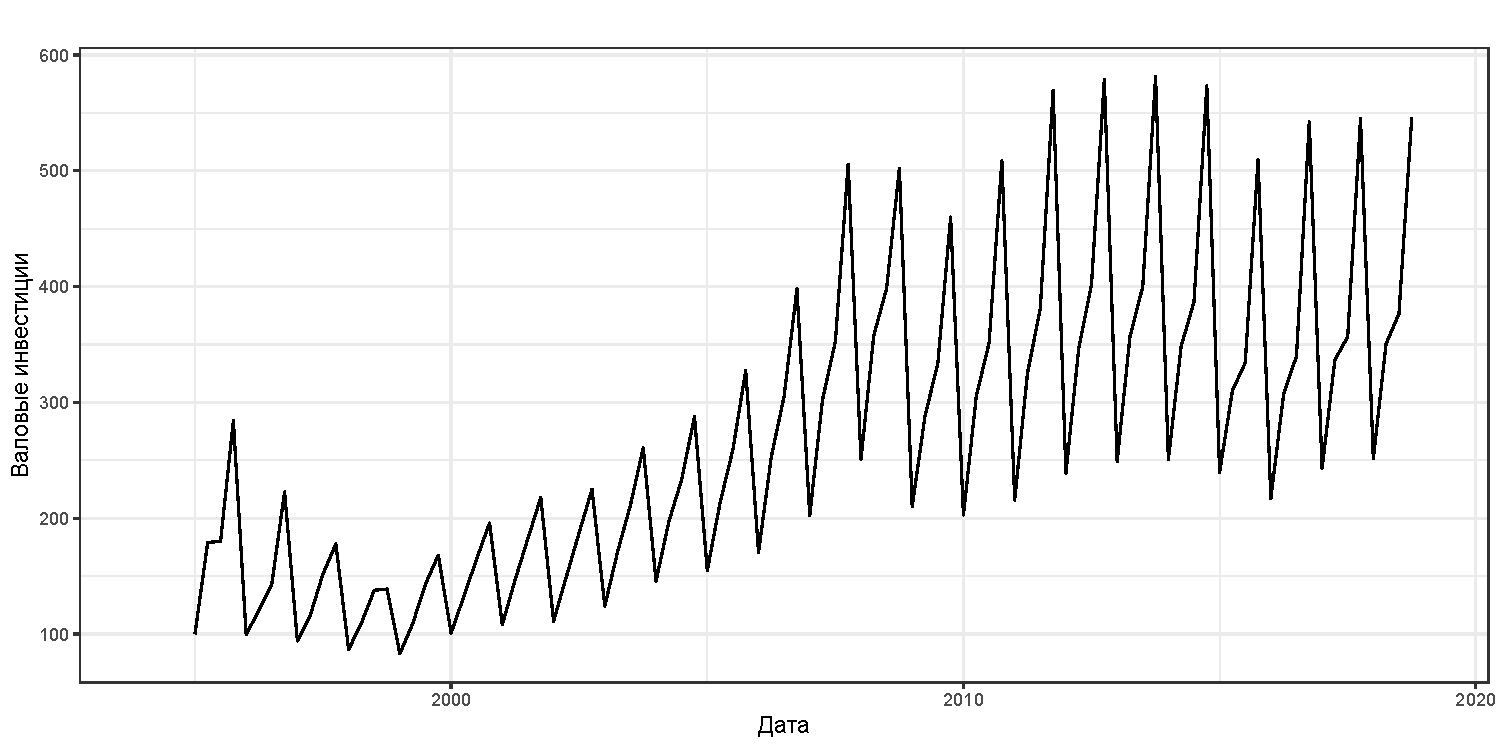
\includegraphics[width = \textwidth]{level_plot.pdf}
    \caption{Валовые инвестиции в России в 1995--2019 гг. в постоянных ценах, в \% к 1-му кварталу 1995 г.}
    \label{fig:level}
\end{figure}

В качестве объясняющих переменных используются 83 российских макроэкономических показателя (квартальные данные,  1-ый квартал 1994 -- 4-ый квартал 2018). Эти показатели отражают состояние экономики, уровень деловой активности, платежного баланса, денежной массы, и т.д. Полный список переменных приведен в приложении \ref{app:list} \footnote{Все данные предоставлены Росстатом:http://www.gks.ru/}.

\section{Дополнительная трансформация данных}
При прогнозировании экономических временных рядов перед тестированием различных моделей часто проводится предварительную трансформацию, например, в виде остационаривания и удаления сезонности. При этом не редко упускается, что, если цель состоит в прогнозировании данных, то нужно учитывать факт нахождения в псевдореальном времени. Например, проводить очистку от сезонности у рядов необходимо удалять только на основании той информации, которые известны на момент составления прогноза. Стандартная трансформация, используемая в работе --- это использование для очистки от сезонности и тренда через взятие четвертой разности логарифма ряда. Использование такой трансформации призвано избежать проблемы, связанной со структурными сдвигами в сезонности.

В отличии от остальных методов построения прогнозов, модель LASSO+VAR не использует для предсказания значения прогнозируемой переменной в момент времени $t+h$ напрямую значения регрессоров в момент времени $t$. Вместо этого прогнозируются значения всех используемых переменных.

%Можно продемонстрировать результаты очистки данных от сезонности с помощью loess на, собственно, объясняемой переменной, уровне валовых инвестиций в России, они приведены на рисунке \ref{fig:des}.

%\begin{figure}[h]
%    \centering
%    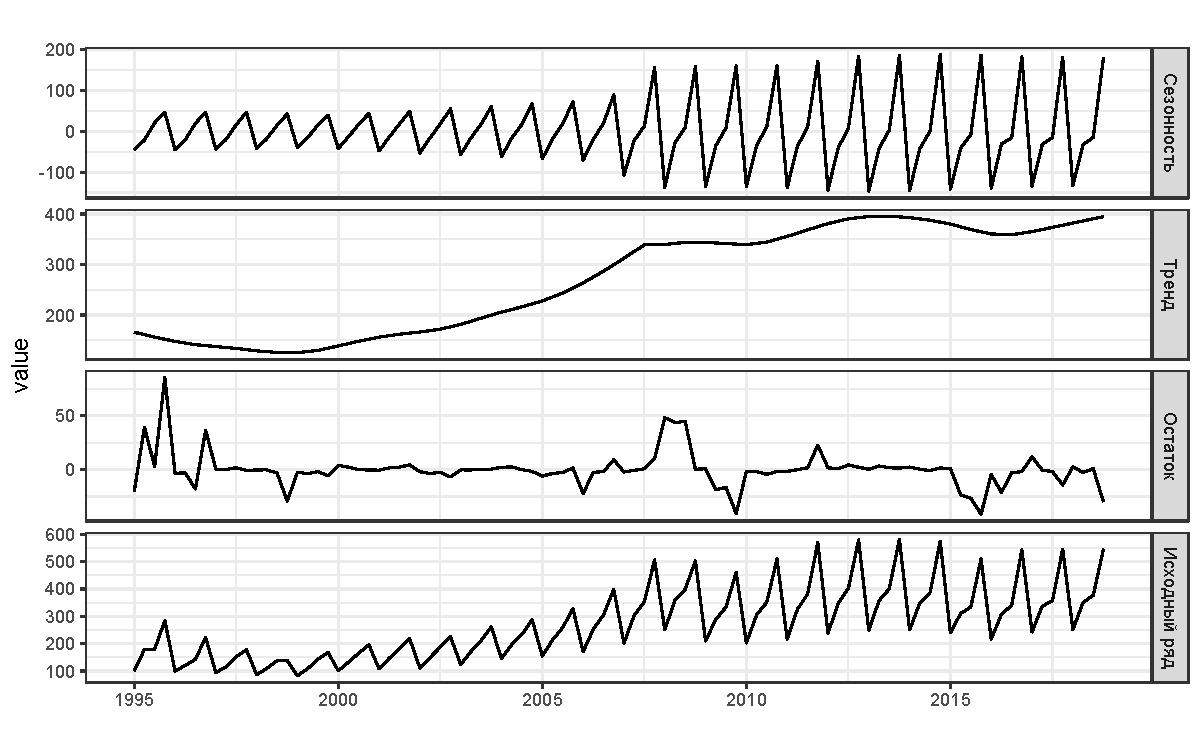
\includegraphics[width = \textwidth]{des_plot.pdf}
%    \caption{Декомпозиция ряда инвестиций}
%    \label{fig:des}
%\end{figure}

\section{Базовая модель}
В качестве базовой модели (фактически цель всех используемых в работе методов --- это превзойти базовую модель по выбранной метрике качества) используется простая акселераторная модель.
Формально модель записывается следующим образом
\begin{equation}
    I_{t+h} =  \mu (Y_{t+h} - Y_{t+h-1}).
\end{equation}
 Для получения предсказаний на $h$ шагов вперед необходимо использовать значения ВВП на $h$ шагов вперед, но т.к. эти значения не могут быть доступны в момент времени $t$, предварительно уровень выпуска оценивается при помощи модели SARIMA$(p,d,q)[4]$, где:
 
 \begin{itemize}
     \item $p$ --- степень лага авторегрессии,
     \item $d$ --- степень дифференцирования процесса,
     \item $q$ --- степень лага случайной ошибки.
     \item $4$ отвечает за сезонность в модели.
 \end{itemize} 
Выбор вектора $(p,  d, q)$ осуществляется при помощи критерия AIC для каждой обучающей выборки отдельно. Отказ от априорного задания параметров обусловлен тем, что структурная форма представления выпуска в виде модели $SARIMA$ могла меняться с 1994 года по 2019 год, и эти изменения необходимо учитывать при составлении прогноза.
\section{Метрики качества}
Главная метрика качества, используемая в модели --- это среднеквадратичная стандартная ошибка (RMSE):
\begin{equation}
  \text{RMSE} = \sqrt{ \frac{\sum_{t = 1}^{T} (\hat{y_t} - y_t)^2}{T}}.
\end{equation}
Такая метрика типична для задач регрессии и, если в разных моделях предсказываются значения регрессантов в одни и те же моменты времени, то эти модели можно с помощью функционала RMSE --- чем больше его значения, тем хуже модель.

Важно отметить, что, поскольку в разных используемых в модели работах предсказываются фактически разные переменные (очищенные или не очищенные предварительно от сезонности), для корректного сравнения всех моделей после получения прогнозов все метрики качества оценивалась на основе четвертых разностей логарифмов прогнозов.

Помимо основной метрики качества RMSE в работе так же для справочной информации рассчитаны и другие метрики качества --- MAE и $R^2$.
MAE показывает средние абсолютные отклонения прогнозов:

\begin{equation}
    \text{MAE} =  \frac{\sum_{t = 1}^{T} |\hat{y_t} - y_t|}{T}.
\end{equation}
$R^2$ показывает долю дисперсии объясняемой переменной, объясненную прогнозными значениями.
\begin{equation}
    R^2 = 1 -\frac{ \sum_{t = 1}^{T}(\hat{y_t} - y_t)^2}{\sum_{t = 1}^{T}(\hat{y_t} - y_t)^2)},
\end{equation}

они приведены в приложении \ref{app:score}.

\section{Построение прогнозов}

Обучение моделей и выбор всех гиперпараметров путем кросс-валидации ведется на десятилетнем скользящем окне (40 наблюдений), проверка качества прогнозирования моделей ведется на тестовой выборке, следующей сразу после тренировочного окна, для изменения валовых инвестиций за период от 1 до 12 кварталов. Важно отметит, что значения гиперпараметров моделей потенциально отличаются для каждой из тренировочных выборок. 

Прогноз строится для отложенной выборки. Это связано с тем, что высокие результаты качества на тренировочной выборке могут говорить о том, что в модели произошло переобучение.

Все вычисления проводились при помощи R.

\chapter{Эмпирические результаты}\label{ch:results}
В этой главе приведены результаты прогнозирования и оценки валовых инвестиций путем использования методов снижения размерности в данных.
\section{Качество моделей}

После получения прогнозных значений для каждой модели были рассчитаны метрики качества. Результаты подсчета RMSE представлены в таблицах \ref{tab:rmse1} для горизонта прогнозирования от 1 до 6 кварталов и \ref{tab:rmse2} для горизонта прогнозирования от 7 до 12 кварталов. В таблицах указаны RMSE соответствующих моделей относительно того же показателя для базовой акселераторной модели. Для справочной информации в приложении \ref{app:score} также приведены другие метрики качества моделей. 



\begin{table}[ht]
\centering
\caption{RMSE для горизонта прогнозирования от 1 до 6 кварталов}
\label{tab:rmse1}
\begin{tabular}{lrrrrrr}
  \hline
Модель & 1 & 2 & 3 & 4 & 5 & 6 \\ 
  \hline
Adaptive LASSO & 0.86 & 0.97 & 1.07 & 1.13 & 1.14 & 1.18 \\ 
  Boosting & 1.96 & 1.36 & 1.11 & 1.01 & 0.87 & 0.82 \\ 
  Elastic Net & 0.87 & 0.97 & 1.04 & 1.10 & 1.10 & 1.10 \\ 
  LASSO & 0.89 & 0.98 & 1.04 & 1.10 & 1.09 & 1.10 \\ 
  LASSO+PC & 0.90 & 0.93 & 1.07 & 1.22 & 1.30 & 1.33 \\ 
  LASSO+VAR & 1.10 & 1.05 & 1.05 & 1.01 & 0.91 & 0.87 \\ 
  Post LASSO & 0.83 & 0.97 & 1.06 & 1.14 & 1.14 & 1.16 \\ 
  Random Forest & 0.96 & 0.93 & 0.95 & 1.02 & 0.96 & 0.96 \\ 
  Ridge & 0.87 & 0.96 & 1.05 & 1.11 & 1.10 & 1.11 \\ 
  Spike and Slab & 0.83 & 0.94 & 1.03 & 1.10 & 1.12 & 1.13 \\ 
   \hline
\end{tabular}
\end{table}

\begin{table}[ht]
\centering
\caption{RMSE для горизонта прогнозирования от 7 до 12 кварталов}
\label{tab:rmse2}
\begin{tabular}{lrrrrrr}
  \hline
Модель & 7 & 8 & 9 & 10 & 11 & 12 \\ 
  \hline
Adaptive LASSO & 1.22 & 1.24 & 1.25 & 1.29 & 1.37 & 1.38 \\ 
  Boosting & 0.80 & 0.82 & 0.77 & 0.74 & 0.74 & 0.75 \\ 
  Elastic Net & 1.12 & 1.14 & 1.14 & 1.15 & 1.19 & 1.20 \\ 
  LASSO & 1.12 & 1.13 & 1.13 & 1.14 & 1.18 & 1.18 \\ 
  LASSO+PC & 1.43 & 1.53 & 1.59 & 1.64 & 1.76 & 1.92 \\ 
  LASSO+VAR & 0.91 & 1.06 & 1.14 & 1.26 & 1.38 & 1.45 \\ 
  Post LASSO & 1.20 & 1.22 & 1.23 & 1.26 & 1.32 & 1.34 \\ 
  Random Forest & 0.97 & 1.02 & 0.96 & 0.96 & 0.97 & 1.01 \\ 
  Ridge & 1.14 & 1.15 & 1.14 & 1.16 & 1.20 & 1.21 \\ 
  Spike and Slab & 1.16 & 1.18 & 1.18 & 1.20 & 1.24 & 1.25 \\ 
   \hline
\end{tabular}
\end{table}

Как видно из таблиц, наилучшее качество для короткого горизонта прогнозирования в 1 или 2 квартала показывают модели Post-LASSO, пик-плато. При этом почти все модели, кроме модели бустинга и LASSO+VAR, показывают результаты хуже, чем акселераторная модель. Однако, начиная с горизонта прогнозирования в 5 кварталов ситуация кардинально меняется и бывшие аутсайдеры (модели бустинга, LASSO+VAR и случайный лес) лидируют и показывают качество лучше, чем у базовой модели. Для горизонта прогнозирования, большего, чем 8 кварталов, никакие другие методы, кроме ансамблевых, не показывают качество лучше, чем у базовой модели. 

Некоторое улучшение качества прогноза моделей с регуляризацией на шаге прогноза, равном 5, может свидетельствовать о наличии авторегрессионной связи ряда валовых инвестиций не только с лагом, равным 4 (эта связь учитывается при удалении из рядов сезонности). Это нужно, видимо, учитывать при построении практического инструментария для прогнозирования инвестиций.

Интересно, что RMSE моделей с регуляризацией почти равномерно повышается с ростом горизонта прогноза относительно RMSE базовой модели, но такой зависимости не наблюдается у ансамблевых методов. На графике \ref{fig:rmse1} показаны значения RMSE для трех базовых моделей с регуляризацией (LASSO, регрессии гребня и регрессии эластичной сети), а на графике \ref{fig:rmse2} --- значения RMSE для модели LASSO ее модификаций. Важно заметить, что улучшения модели LASSO и другие модели с регуляризацией почти никогда не показывали результаты лучшие, чем сама модель LASSO. Стоит признать, что модификации этой модели, потенциально ухудшающие интерпретируемость коэффициентов в обмен на состоятельность оценок, в данной работе ещё и оказались на большинстве горизонтов прогнозирования ещё и хуже простой модели с регуляризацией (LASSO), которая в целом показывает довольно плохие результаты при горизонте прогнозирования меньшем, чем 3 квартала.  В то же время модели эластичной сети и регрессии гребня, хотя и демонстрирует стабильно худшее качество, чем модель LASSO, всё же находится близко к ней.

\begin{figure}[h]
    \centering
    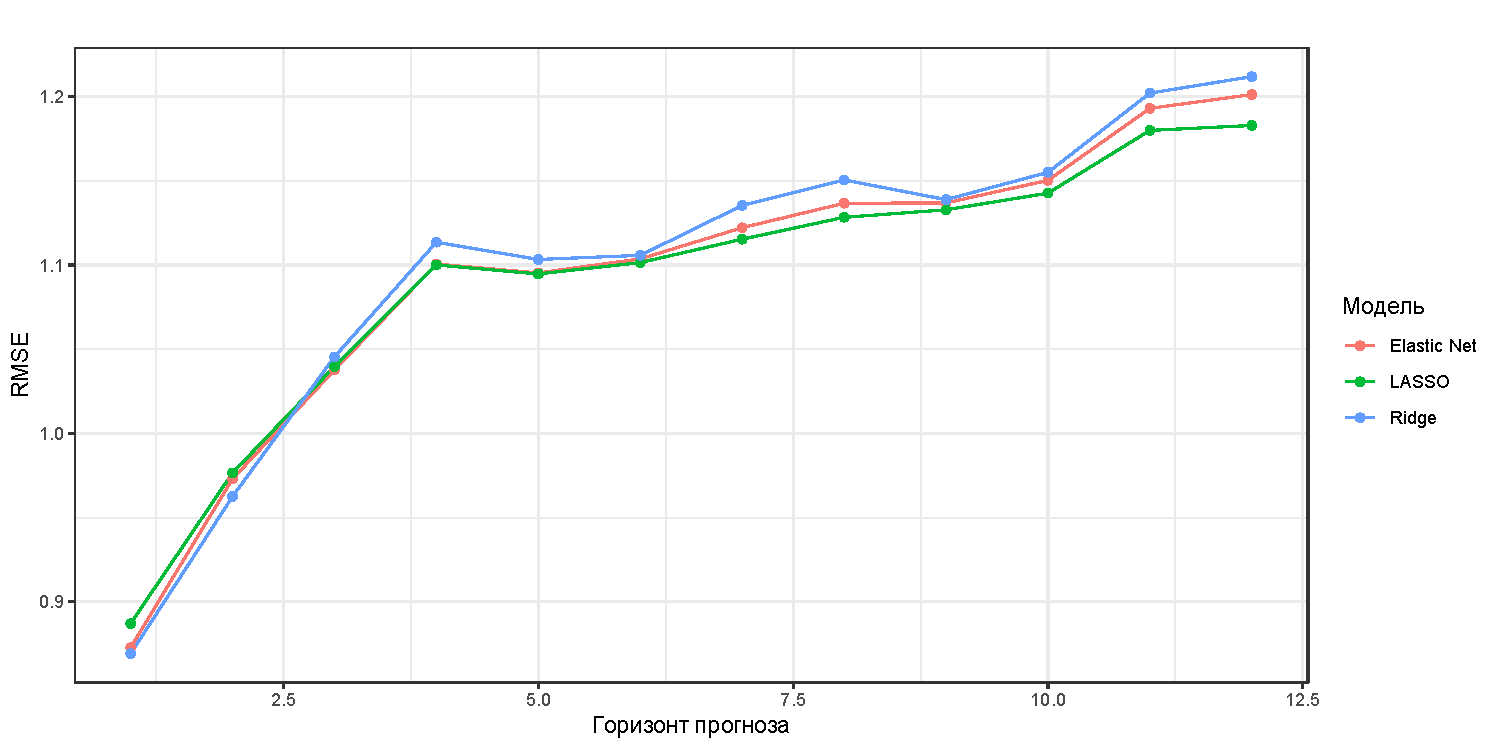
\includegraphics[width = \textwidth]{rmse1.pdf}
    \caption{RMSE прогнозов относительно акселераторной модели}
    \label{fig:rmse1}
\end{figure}


\begin{figure}[h]
    \centering
    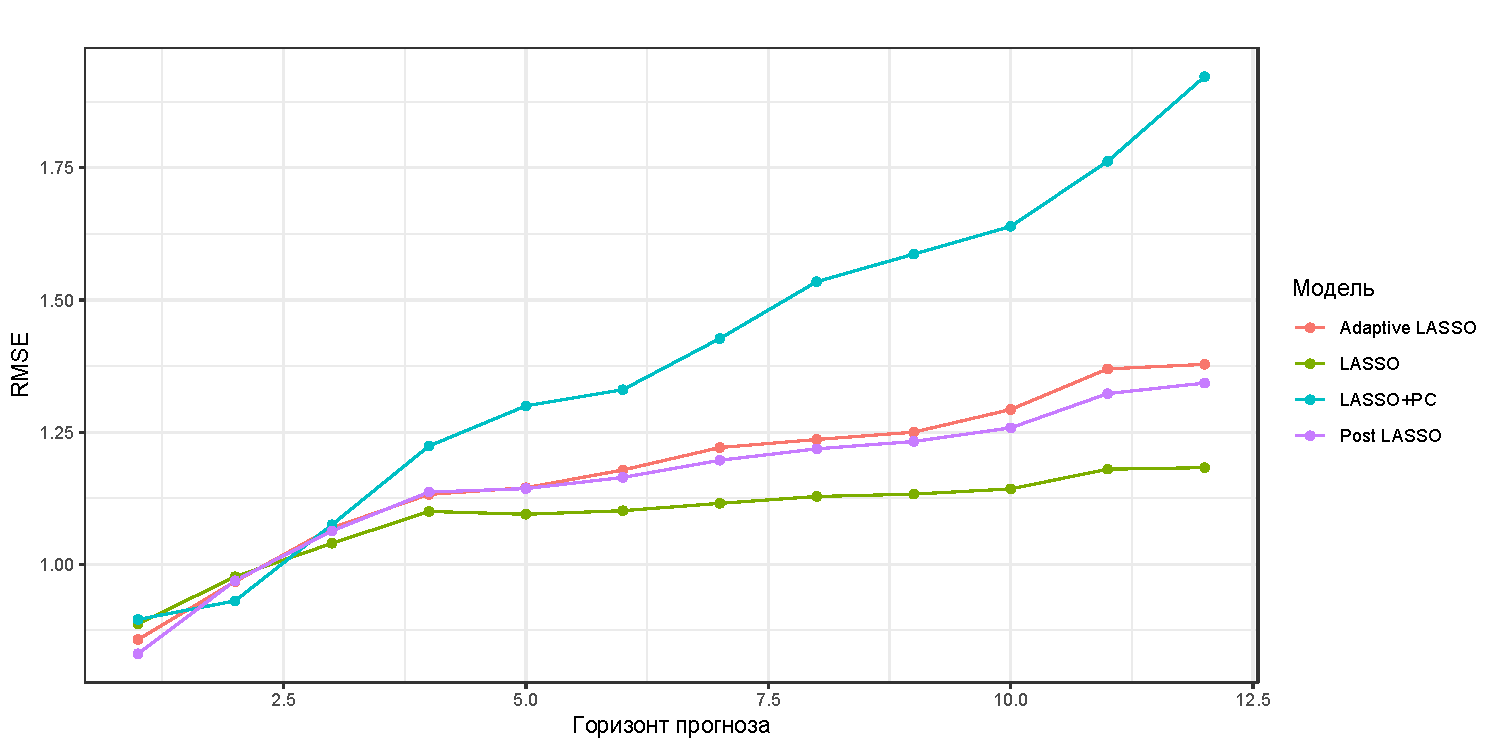
\includegraphics[width = \textwidth]{rmse2.pdf}
    \caption{RMSE прогнозов относительно акселераторной модели}
    \label{fig:rmse2}
\end{figure}

Стоит также отметить, что байесовская модель (пик-плато), хотя и не лидирует среди остальных моделей ни для одного из горизонтов прогнозирования, в целом показывает лучшие результаты, чем модель LASSO. Это кажется важным результатом, если учесть, что модели бустинга и случайного леса довольно плохо интерпретируются, в то время как использование байесовской регрессии пик-плато позволяет говорить об условной вероятности присутствия тех или иных переменных в модели. 

На рисунке \ref{fig:rmse3} можно видеть, что в среднем модели бустинга, случайного леса и регрессии пик-плато показывают стабильное качество при горизонте прогноза, большем 4. На начальном этапе из этих трех моделей, стоящих особняком от моделей регуляризации, лидирует регрессия пик-плато, а на более длинных промежутках прогнозирования --- бустинг. Это согласуется с тем, что регрессия пик-плато фактически представляет собой байесовский аналог регуляризации. В целом можно выявить такую закономерность: при малом количестве наблюдений простые модели с регуляризацией (LASSO и некоторые модификации) и байесовские аналоги регуляризацией (пик-плато) показывают при задаче прогнозирования инвестиций в России относительно качество, но, с ростом горизонта прогноза, их качество ухудшается относительно модели бустинга. 

Эмпирически бустинг показывает отличные результаты, как правило, при большом количестве наблюдений, и таким образом, результаты данной работы ценны тем, что показывают: даже при малом количестве наблюдений модель бустинга позволяет получать на больших горизонтах прогноза, когда, казалось бы, ничего лучше кроме наивного прогноза быть не может, результаты лучше, чем у стандартных моделей инвестиций.


\begin{figure}[h]
    \centering
    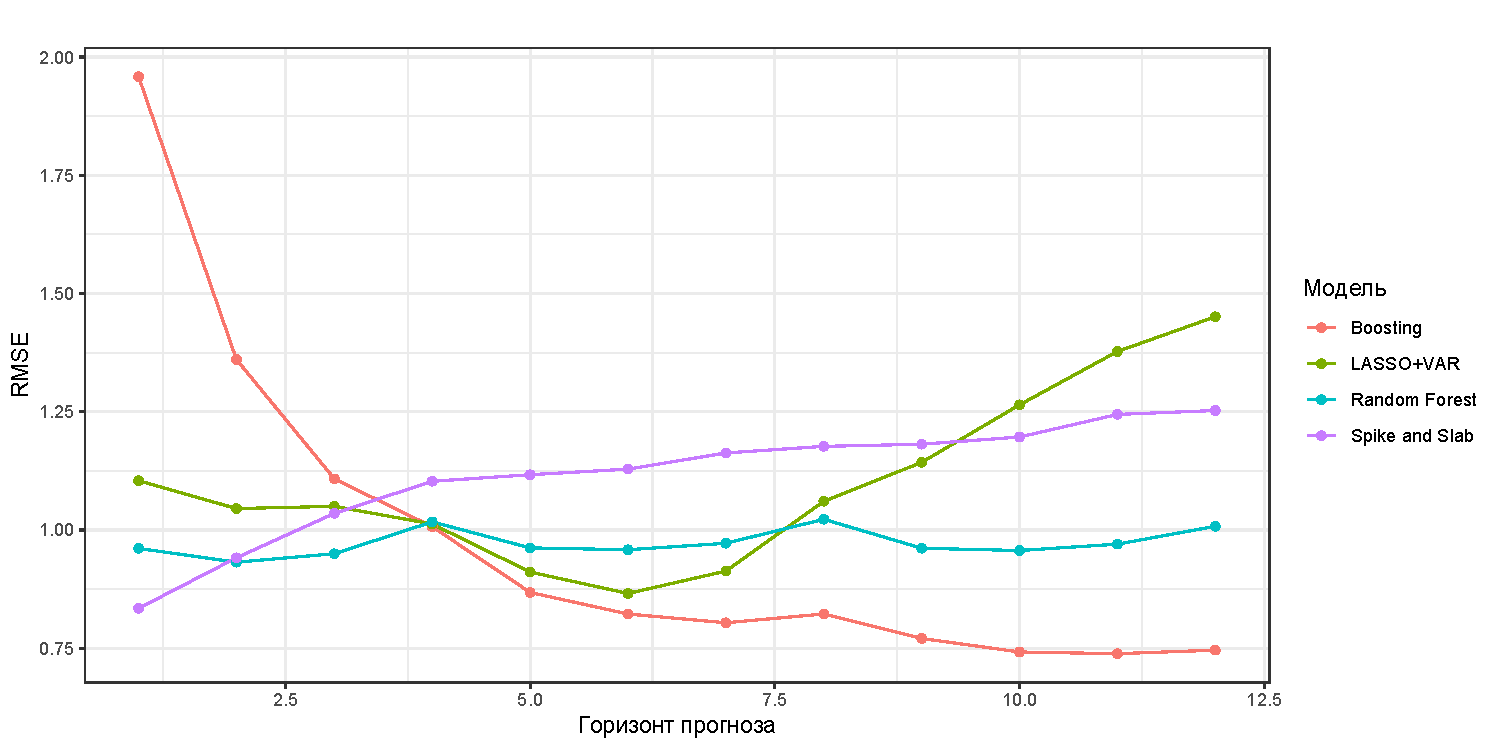
\includegraphics[width = \textwidth]{rmse3.pdf}
    \caption{RMSE прогнозов относительно акселераторной модели}
    \label{fig:rmse3}
\end{figure}
\begin{figure}[h]
    \centering
    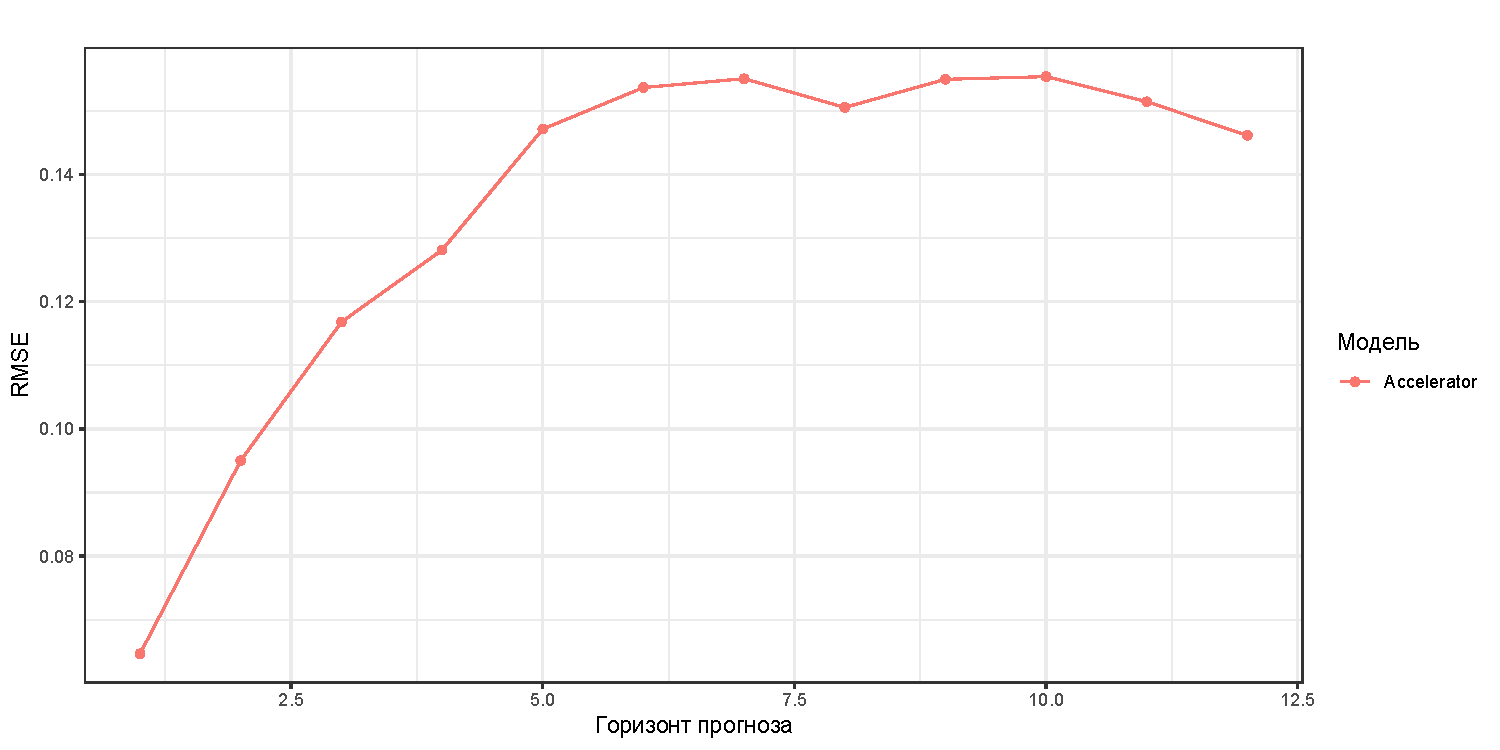
\includegraphics[width = \textwidth]{rmse4.pdf}
    \caption{RMSE акселераторной модели}
    \label{fig:rmse4}
\end{figure}




В целом можно отметить, что с ростом горизонта прогнозирования ожидаемо в среднем падает качество всех моделей, у одних --- значительно, у других --- не так сильно. Сам факт падения качества, очевидно, объясняется отдаление от даты прогноза. С ростом промежутка, через который производится прогнозирование, растет количество случайных шоков, которые учесть невозможно и которые при этом отрицательно повлияют на качество прогнозов. Интересен не сам факт падения качества, а характер этого падения. На рисунке \ref{fig:rmse4} показан RMSE акселераторной модели. Можно заметить, что для модели бустинга характерно относительно умеренное улучшение качества относительно базовой модели с ростом горизонта прогноза, в то время как для моделей с регуляризацией характерно взрывное падение качества с ростом горизонта прогноза. В то же время сравнивая модели обычной регуляризации (LASSO) и байесовской (пик-плато), стоит отдать предпочтение последней из-за относительно стабильности качества (хоть последнее и не всегда превышает качество базовой модели).


\section{Прогнозы}
Помимо исследования качества моделей, интересно смотреть и на, собственно, сами прогнозы. Учитывая, что в ряду инвестиций присутствует сильная сезонность, графики, собственно, самих предсказаний сообщили бы мало информации. Поэтому логично рассматривать графики годовых средних прогнозов. На рисунке \ref{fig:smooth1} можно видеть сглаженные прогнозы для простых моделей с регуляризацией в сравнении с исходным глаженным рядом и сглаженным прогнозом модели акселератора. Что можно понять из этих графиков? Во-первых, большинство моделей в целом показывают прогнозы, очень схожие с моделью акселератора.

В 2007 -- 2008 годах наблюдается спад инвестиций в России в связи с мировым кризисом. Все модели не очень хорошо реагируют на этот спад (они не могут его хорошо предсказать на больших горизонтах прогнозирования, и, более того, уже после кризиса, когда инвестиции возвращаются на прежний уровень, они прогнозирует как раз спад). Примерно после 2010 года при малом горизонте прогнозирования, модели с регуляризацией довольно точно предсказывают значений инвестиций, но при больших горизонтах прогнозирования, видимо, происходит переобучение и прогнозы довольно сильно отдаляются от настоящих значений.


Что происходит в случае модификаций модели LASSO? На рисунке \ref{fig:smooth2} показаны сглаженные прогнозы для этих моделей в сравнении с базовой моделью и настоящими значениями. В целом ситуация повторяется (большую проблему представляет запаздывающие предсказание кризиса, приводящее к большим ошибкам в моделях), но фактически переобучение, ведущие к большим колебаниям вокруг истинных значений прогнозируемого ряда) у моделей-модификаций LASSO происходит драматичнее.


Любопытно, что при достаточно больших горизонтах модели с регуляризацией неплохо предсказывают падение инвестиций и дальнейшую стагнацию экономики в 2014--2015 годах
\begin{figure}[h]
    \centering
    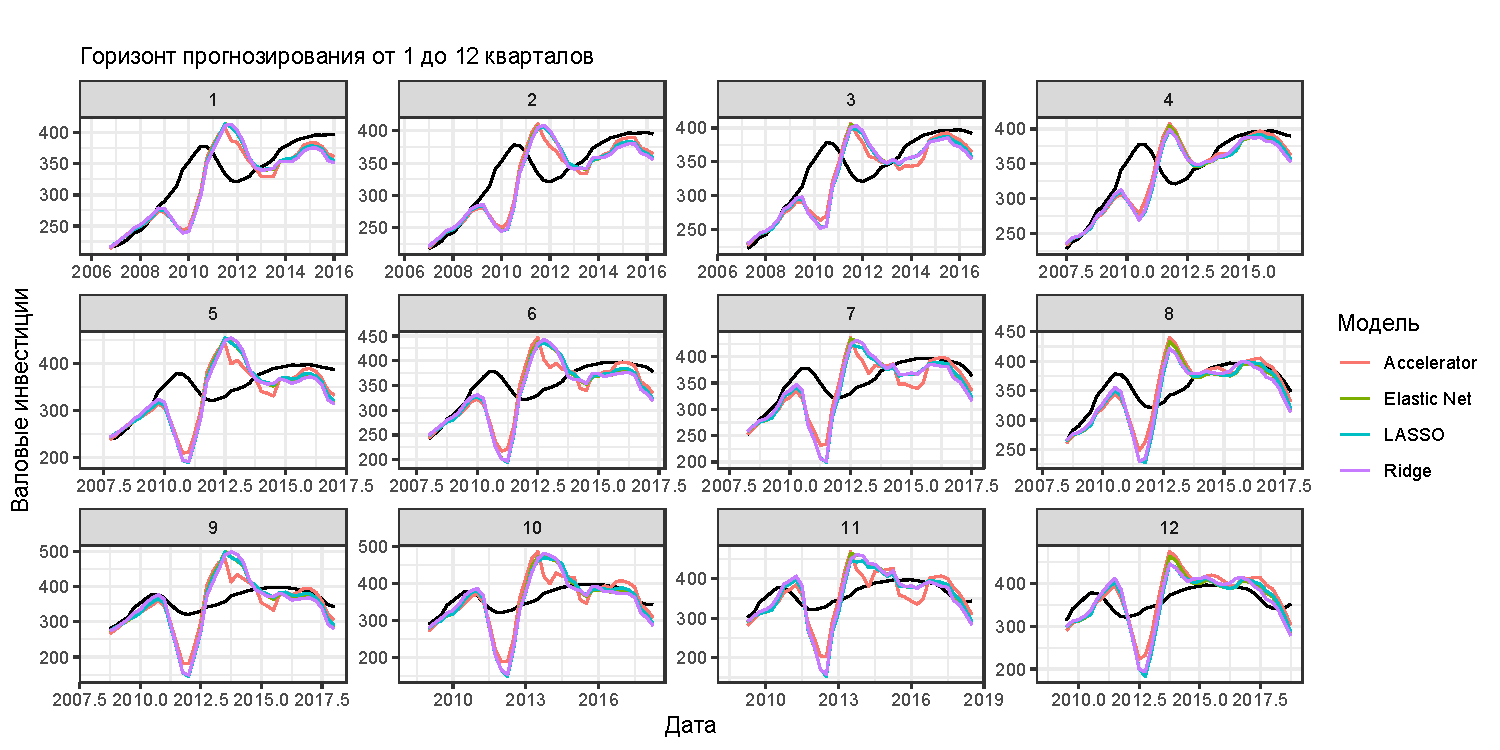
\includegraphics[width = \textwidth]{smooth1.pdf}
    \caption{Прогнозы валовых инвестиций, годовое сглаживание}
    \label{fig:smooth2}
\end{figure}

\begin{figure}[h]
    \centering
    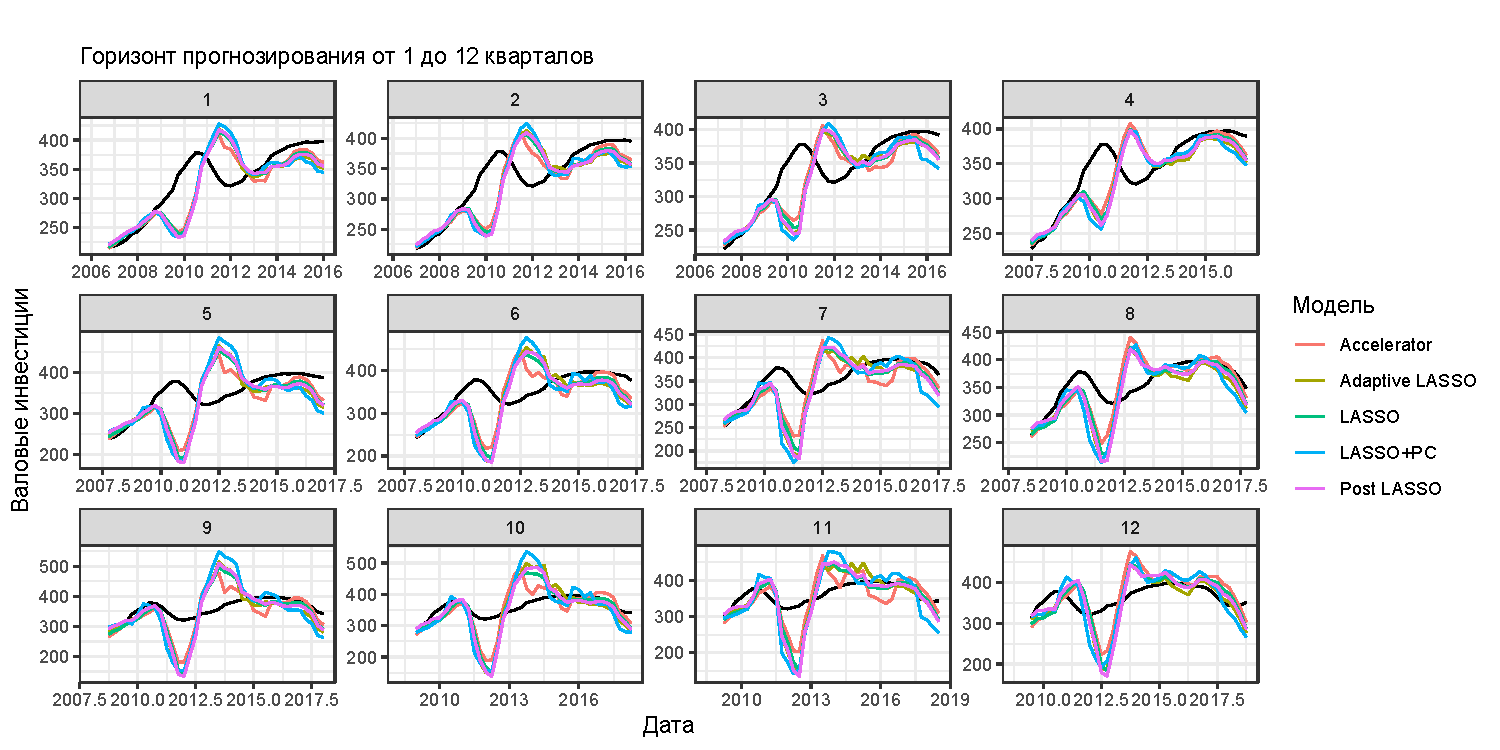
\includegraphics[width = \textwidth]{smooth2.pdf}
    \caption{Прогнозы валовых инвестиций, годовое сглаживание}
    \label{fig:smooth1}
\end{figure}

Стоит обратится и к прогнозам других моделей. На рисунке \ref{fig:smooth3} показаны прогнозы для моделей случайного леса, бустинга, пик-плато в сравнении с базовой моделью и истинными значениями инвестиций. Можно заметить, что успех модели бустинга обеспечен умеренной реакцией на кризис 2008 года и такой же умеренной реакцией на дальнейший рост экономики. Бустинг лучше, чем другие модели, реагировал на изменения в ходе кризиса и поэтому прогнозы на период посткризисного восстановления оказались не столь далеки от реальности. В то же время бустинг прогнозировал значительный прирост инвестиций в период кризиса 2014--2015 года, что привело к ухудшению качества модели.

Модель LASSO+VAR продемонстрировала хорошие результаты на средних горизонтах прогнозирования (5---7 кварталов) и плохие на коротких и длинных, что не типично для остальных моделей. Было бы любопытно посмотреть детальнее, что же к этому привело. На рисунке \ref{fig:smooth4} приведен график прогнозов в сравнении с прогнозами базовой модели и истинных значений. Можно видеть в целом сходство с моделью акселератора для коротких предсказаний и прогнозируемый на длинных промежутках взрывной рост инвестиций прямо во время кризиса 2007--2008 годов. Модель продемонстрировала опасную склонность к переобучению. 

Обобщая данный параграф, можно с удовлетворением заметить, что ни одна из тех моделей, которые показали хорошие результаты на больших горизонтах прогнозирования, не получила эти результаты благодаря выбору наивного прогноза. 

Во-первых, это значит, что в рассматриваемый период существовали некоторые неявные закономерности, позволяющие давать относительно хорошие прогнозы уровня инвестиций в России, и наивный прогноз, который бы рассматривал процесс изменения инвестиций в виде случайного блуждания, оказался не слишком хорош. Ниже будут рассмотрены возможные примеры таких закономерностей.


\begin{figure}[h]
    \centering
    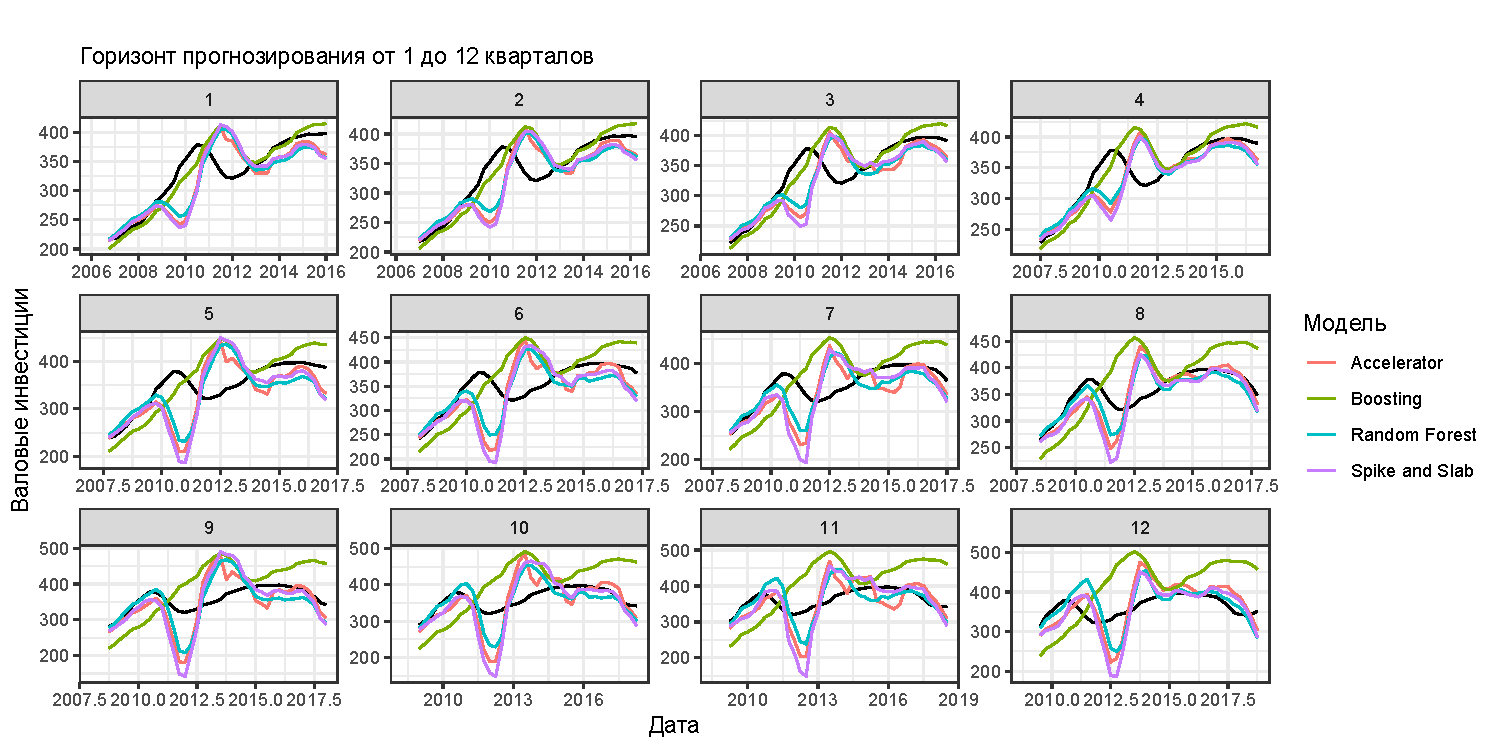
\includegraphics[width = \textwidth]{smooth3.pdf}
    \caption{Прогнозы валовых инвестиций, годовое сглаживание}
    \label{fig:smooth3}
\end{figure}


\begin{figure}[h]
    \centering
    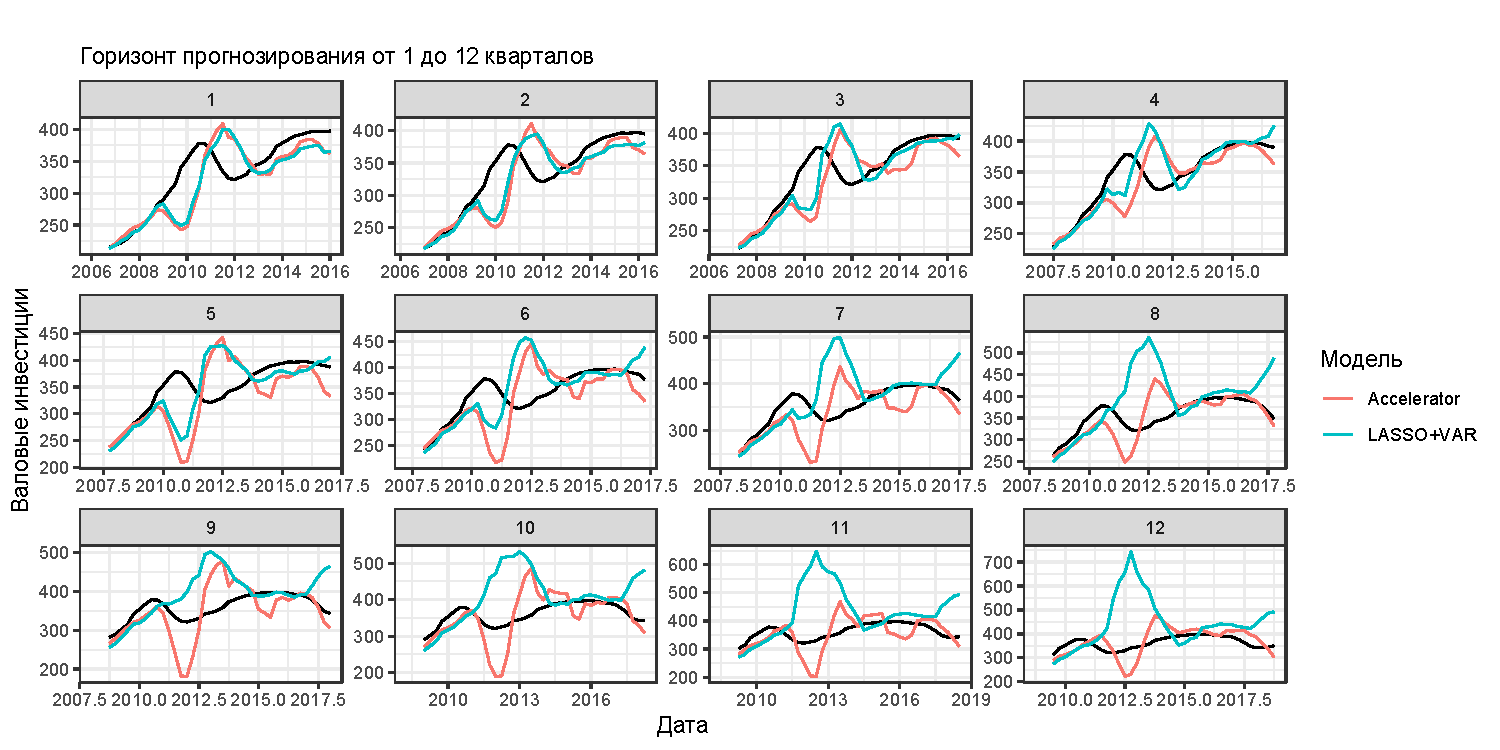
\includegraphics[width = \textwidth]{smooth4.pdf}
    \caption{Прогнозы валовых инвестиций, годовое сглаживание}
    \label{fig:smooth4}
\end{figure}
\section{Ошибки моделей}
Важную часть анализа результатов применения моделей занимает анализ ошибок этих моделей. Фактически, если в результате построения прогнозов ошибки оказались например, систематически смещены от нуля, уже нельзя говорить о несмещенности коэффициентов в линейных моделях. Кроме того, сомнительны будут любые утверждения о качестве моделей, т.к. полученные результаты могут быть связаны со структурой данных и сильно поменяются, если данные окажутся другими. На рисунке \ref{fig:error1} можно видеть графики распределения ошибок прогнозов для простых моделей с регуляризацией. В целом графики очень похожи в совпадающие горизонты прогнозирования.

\begin{figure}[h]
    \centering
    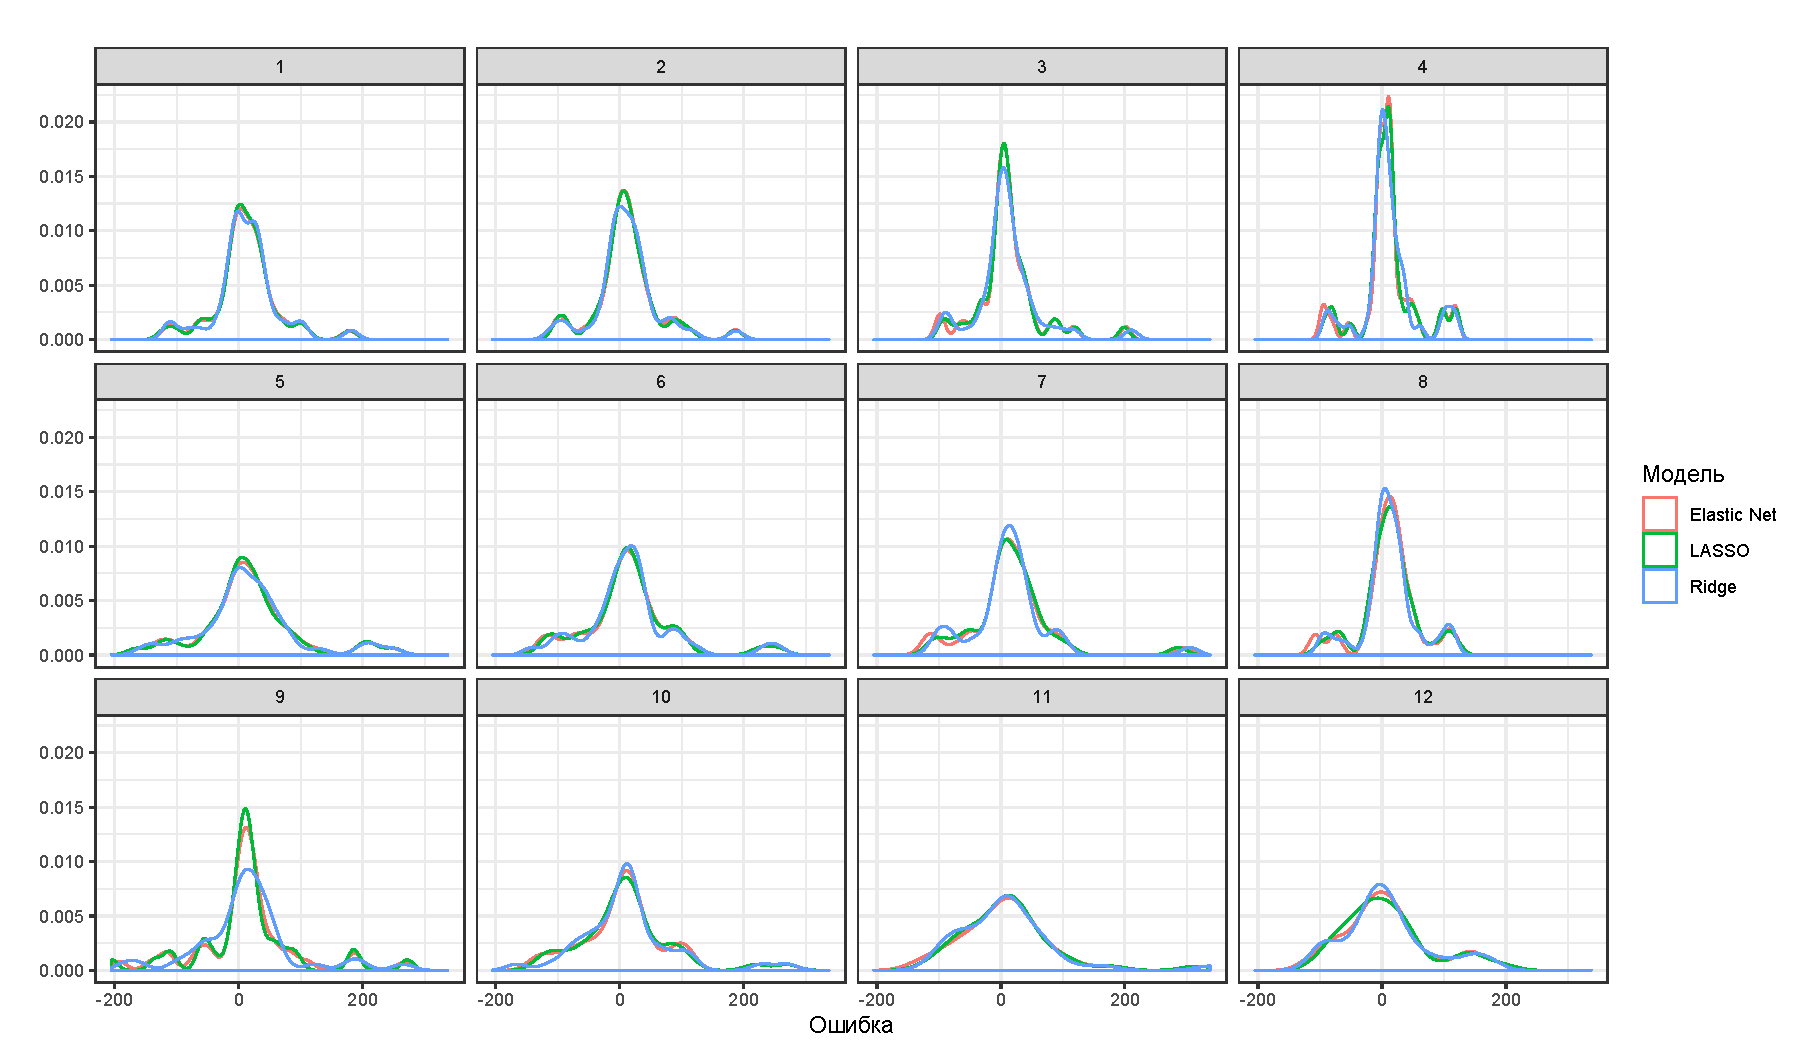
\includegraphics[width = \textwidth]{error1.pdf}
    \caption{Плотность распределения ошибок}
    \label{fig:error1}
\end{figure}
На рисунке \ref{fig:error2} можно видеть графики распределения ошибок прогнозов для модели LASSO и ее модификаций. В целом графики очень похожи в совпадающие горизонты прогнозирования. Фактически только в случае LASSO и Adaptive LASSO можно предполагать нормальность ошибок (ниже эти предположения будут проверены), в то время как распределение ошибок для других моделей демонстрирует скошенность и смещенность.


\begin{figure}[h]
    \centering
    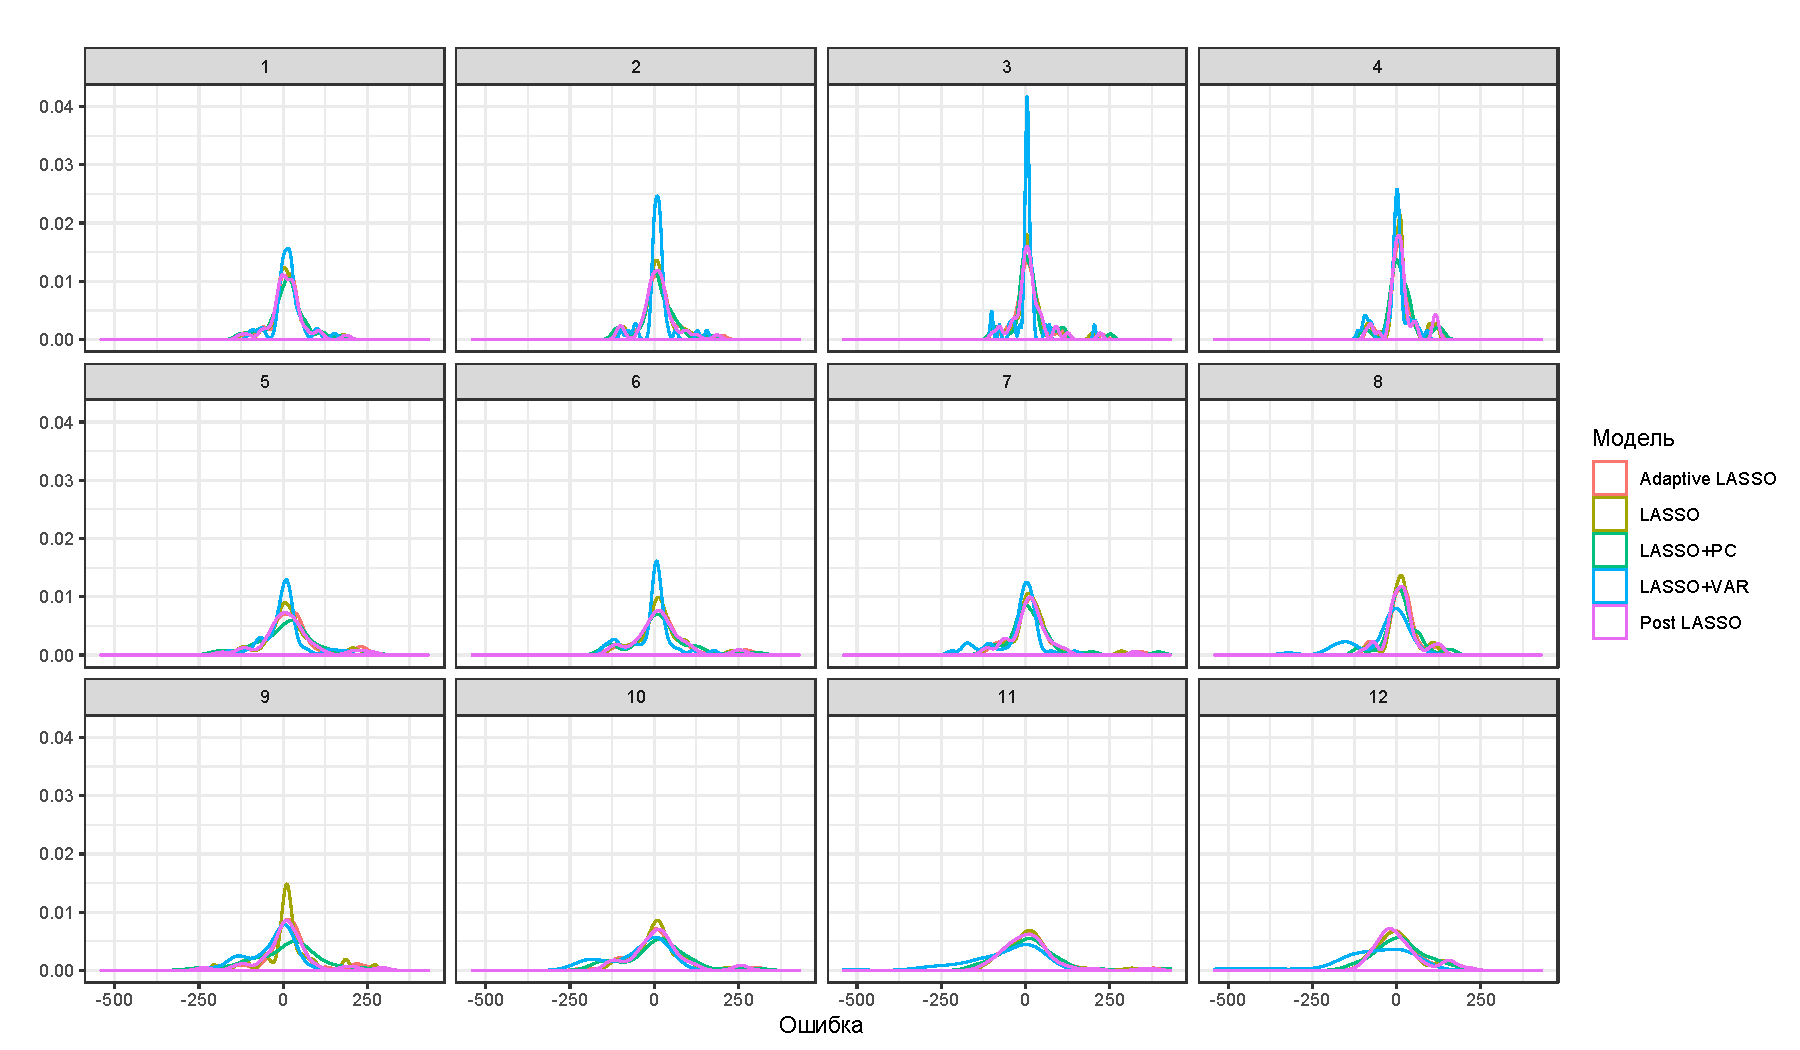
\includegraphics[width = \textwidth]{error2.pdf}
    \caption{Плотность распределения ошибок}
    \label{fig:error2}
\end{figure}


Наконец, на рисунке \ref{fig:error3} можно видеть графики распределения ошибок прогнозов для моделей бустинга, случайного леса и пик-плато. Можно заметить систематическое смещение пика распределения ошибок для метода случайного леса влево. Это говорит о том что в среднем прогнозы случайного леса были ниже, чем истинные значения.
\begin{figure}[h]
    \centering
    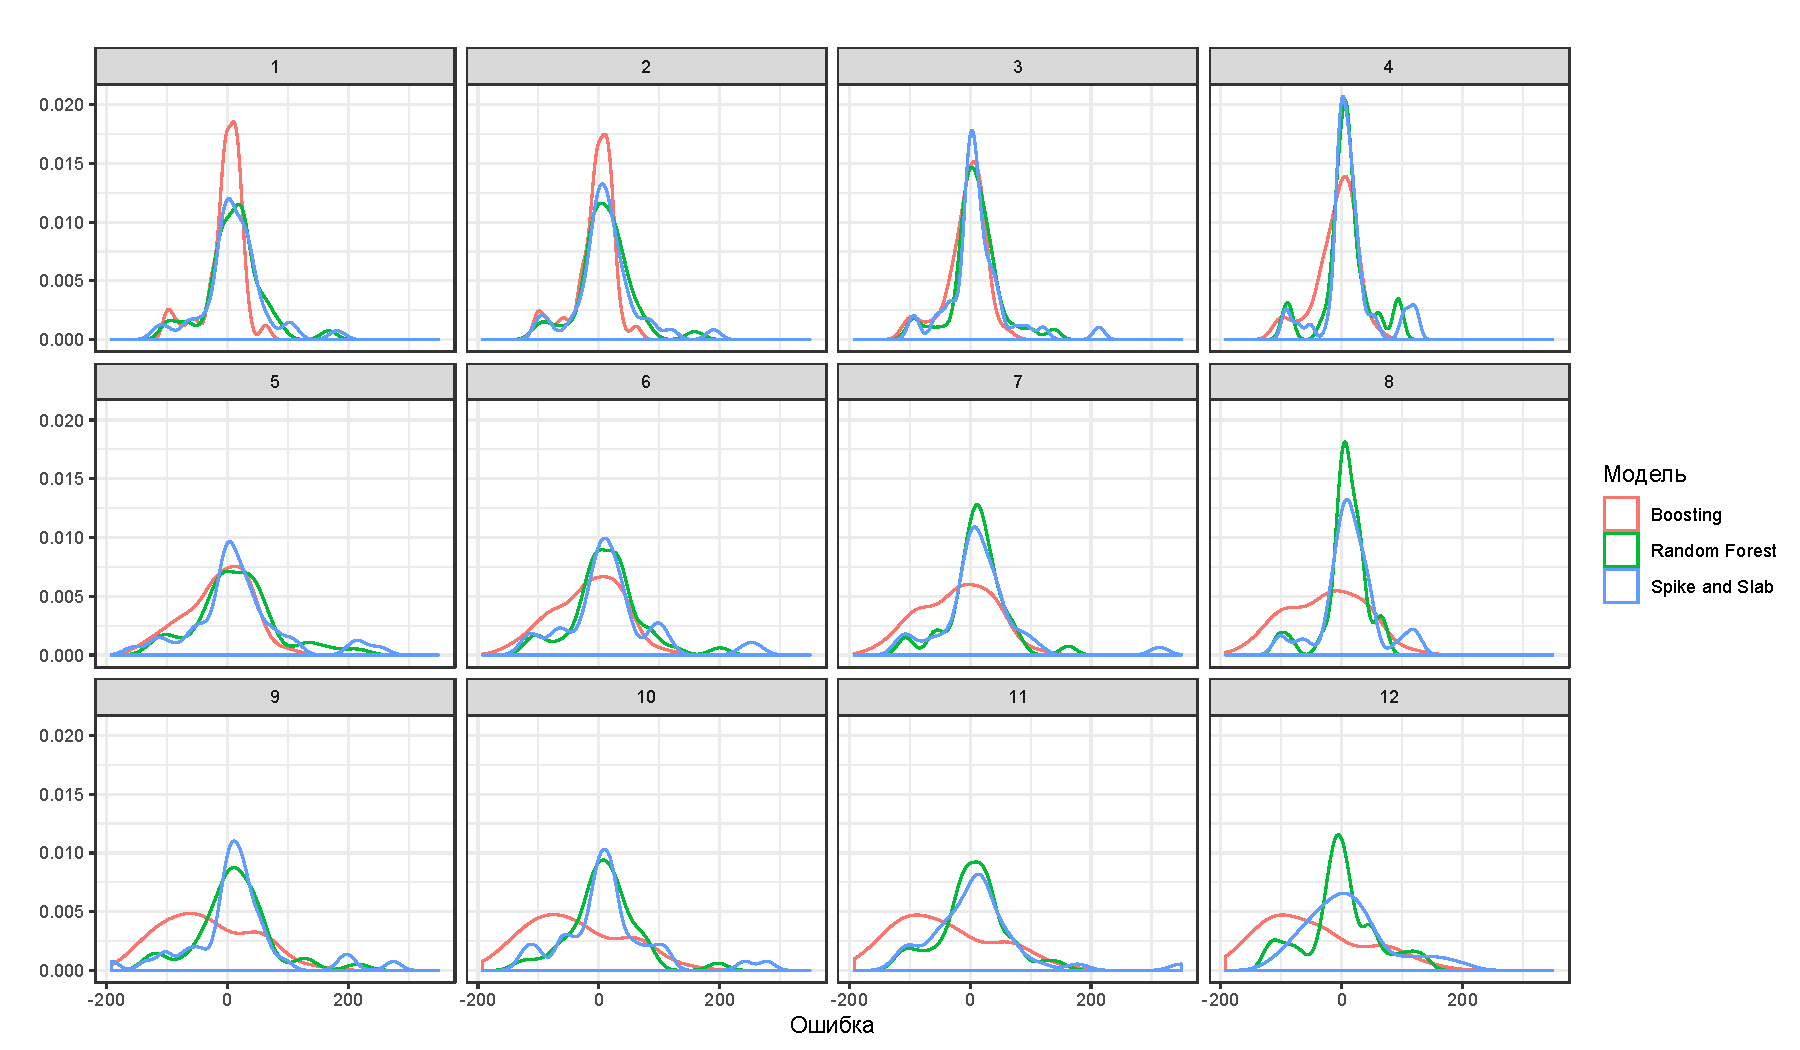
\includegraphics[width = \textwidth]{error3.pdf}
    \caption{Плотность распределения ошибок}
    \label{fig:error3}
\end{figure}

Далее рассмотрены результаты тестирования ошибок на нормальность при помощи критерия Шапиро-Уилка. Критерий Шапиро-Уилка проверяет гипотезу $H_0:$ <<случайная величина X распределена нормально>>. Статистика критерия имеет вид:
\begin{equation}
    W = \frac{1}{S^2\left(\sum_{i=1}^n a(n-i+1) (x_{n-i+1} - x_i)\right)^2},
\end{equation}
где:

\begin{itemize}
    \item $S^2 = \sum_{i=1}^{n} \left(x_i = \bar{x}\right)^2$
    \item $a(n)$ --- коэффициент, зависящий от размера выборки
\end{itemize}
Данный критерий описан в работе \cite{shapiro1965analysis}
Результаты проверки критерия отдельно для каждой модели и каждого горизонта прогнозирования представлены в таблице \ref{tab:er1} (для горизонтов прогнозирования от 1 до 6 кварталов) и \ref{tab:er2} (для горизонтов прогнозирования от 7 до 12 кварталов). В целом можно с удовлетворением заметить, что для фаворита работы --- модели бустинга, начиная с 5 квартала горизонта прогнозирования, гипотеза о нормальности ошибок не отвергается, в отличии от остальных моделей, демонстрирующих отсутствие нормальности почти для каждого горизонта.

\begin{table}[ht]
\centering
\caption{Проверка ошибок на нормальность для горизонта от 1 до 6 кварталов}
\label{tab:er1}
\begin{tabular}{lrrrrrr}
  \hline
Модель & 1 & 2 & 3 & 4 & 5 & 6 \\ 
  \hline
Adaptive LASSO & 0.01 & 0.01 & 0.00 & 0.00 & 0.00 & 0.00 \\ 
  Boosting & 0.00 & 0.00 & 0.00 & 0.00 & 0.25 & 0.45 \\ 
  Elastic Net & 0.01 & 0.01 & 0.00 & 0.00 & 0.01 & 0.00 \\ 
  LASSO & 0.01 & 0.00 & 0.00 & 0.00 & 0.01 & 0.00 \\ 
  LASSO+PC & 0.18 & 0.02 & 0.00 & 0.00 & 0.14 & 0.01 \\ 
  LASSO+VAR & 0.00 & 0.00 & 0.00 & 0.00 & 0.00 & 0.00 \\ 
  Post LASSO & 0.01 & 0.00 & 0.00 & 0.00 & 0.01 & 0.00 \\ 
  Random Forest & 0.02 & 0.01 & 0.01 & 0.00 & 0.06 & 0.04 \\ 
  Ridge & 0.01 & 0.00 & 0.00 & 0.00 & 0.01 & 0.00 \\ 
  Spike and Slab & 0.01 & 0.00 & 0.00 & 0.00 & 0.00 & 0.00 \\ 
   \hline
\end{tabular}
\end{table}


\begin{table}[ht]
\centering
\caption{Проверка ошибок на нормальность для горизонта от 7 до 12 кварталов}
\begin{tabular}{lrrrrrr}
  \hline
Модель & 7 & 8 & 9 & 10 & 11 & 12 \\ 
  \hline
Adaptive LASSO & 0.00 & 0.04 & 0.00 & 0.00 & 0.00 & 0.02 \\ 
  Boosting & 0.55 & 0.54 & 0.23 & 0.19 & 0.14 & 0.09 \\ 
  Elastic Net & 0.00 & 0.00 & 0.00 & 0.01 & 0.00 & 0.06 \\ 
  LASSO & 0.00 & 0.03 & 0.00 & 0.00 & 0.00 & 0.01 \\ 
  LASSO+PC & 0.00 & 0.04 & 0.17 & 0.15 & 0.00 & 0.84 \\ 
  LASSO+VAR & 0.00 & 0.00 & 0.00 & 0.00 & 0.00 & 0.00 \\ 
  Post LASSO & 0.00 & 0.03 & 0.00 & 0.00 & 0.00 & 0.00 \\ 
  Random Forest & 0.01 & 0.00 & 0.02 & 0.07 & 0.28 & 0.09 \\ 
  Ridge & 0.00 & 0.01 & 0.00 & 0.00 & 0.00 & 0.04 \\ 
  Spike and Slab & 0.00 & 0.01 & 0.00 & 0.00 & 0.00 & 0.04 \\ 
   \hline
\end{tabular}
\end{table}


\section{Ненулевые коэффициенты}
Задача прогнозирования, конечно, очень важна, но, помимо построения прогнозов, интересно было бы также интерпретировать полученные зависимости. Надо отметить, что использование методов снижения размерности в некотором смысле подразумевает движение в обратную сторону от традиционного способа экономического анализа:


\begin{itemize}
    \item Построение гипотез на основе теории
\item Проверка гипотез на имеющихся данных
\end{itemize}
Конечно, было бы неосмотрительно и глупо спорить с этими устоявшимися представлениями о том, как должно выглядеть экономическое исследование, однако же, было бы любопытно посмотреть, что в качестве лучших объясняющих переменных выдают своеобразные <<черные ящики>> --- модели с регуляризацией. В этом разделе не рассматриваются полученные в моделях случайного леса и бустинга зависимости, т.к. они довольно плохо интерпретируются.

На рисунке \ref{fig:lp2} отображена доля включений различных использованных в работе переменных в качестве переменных в модели LASSO, а в \ref{fig:lp1} --- для модели Adaptive LASSO. Здесь следует напомнить, что эти две модели отличаются тем, что в последней в функции штрафа переменным задаются веса (по аналогии с обобщённым методом наименьших квадратов можно было бы назвать Adaptive LASSO обобщённым методом LASSO). Хотя на конкретных данных в этой работе последняя показала худшие результаты, чем просто модель LASSO, коэффициенты в ней выбираются более обоснованно и оценки их состоятельны, поэтому было бы интересно сравнить, какие переменные отобрали эти две модели.
\begin{figure}[h]
    \centering
    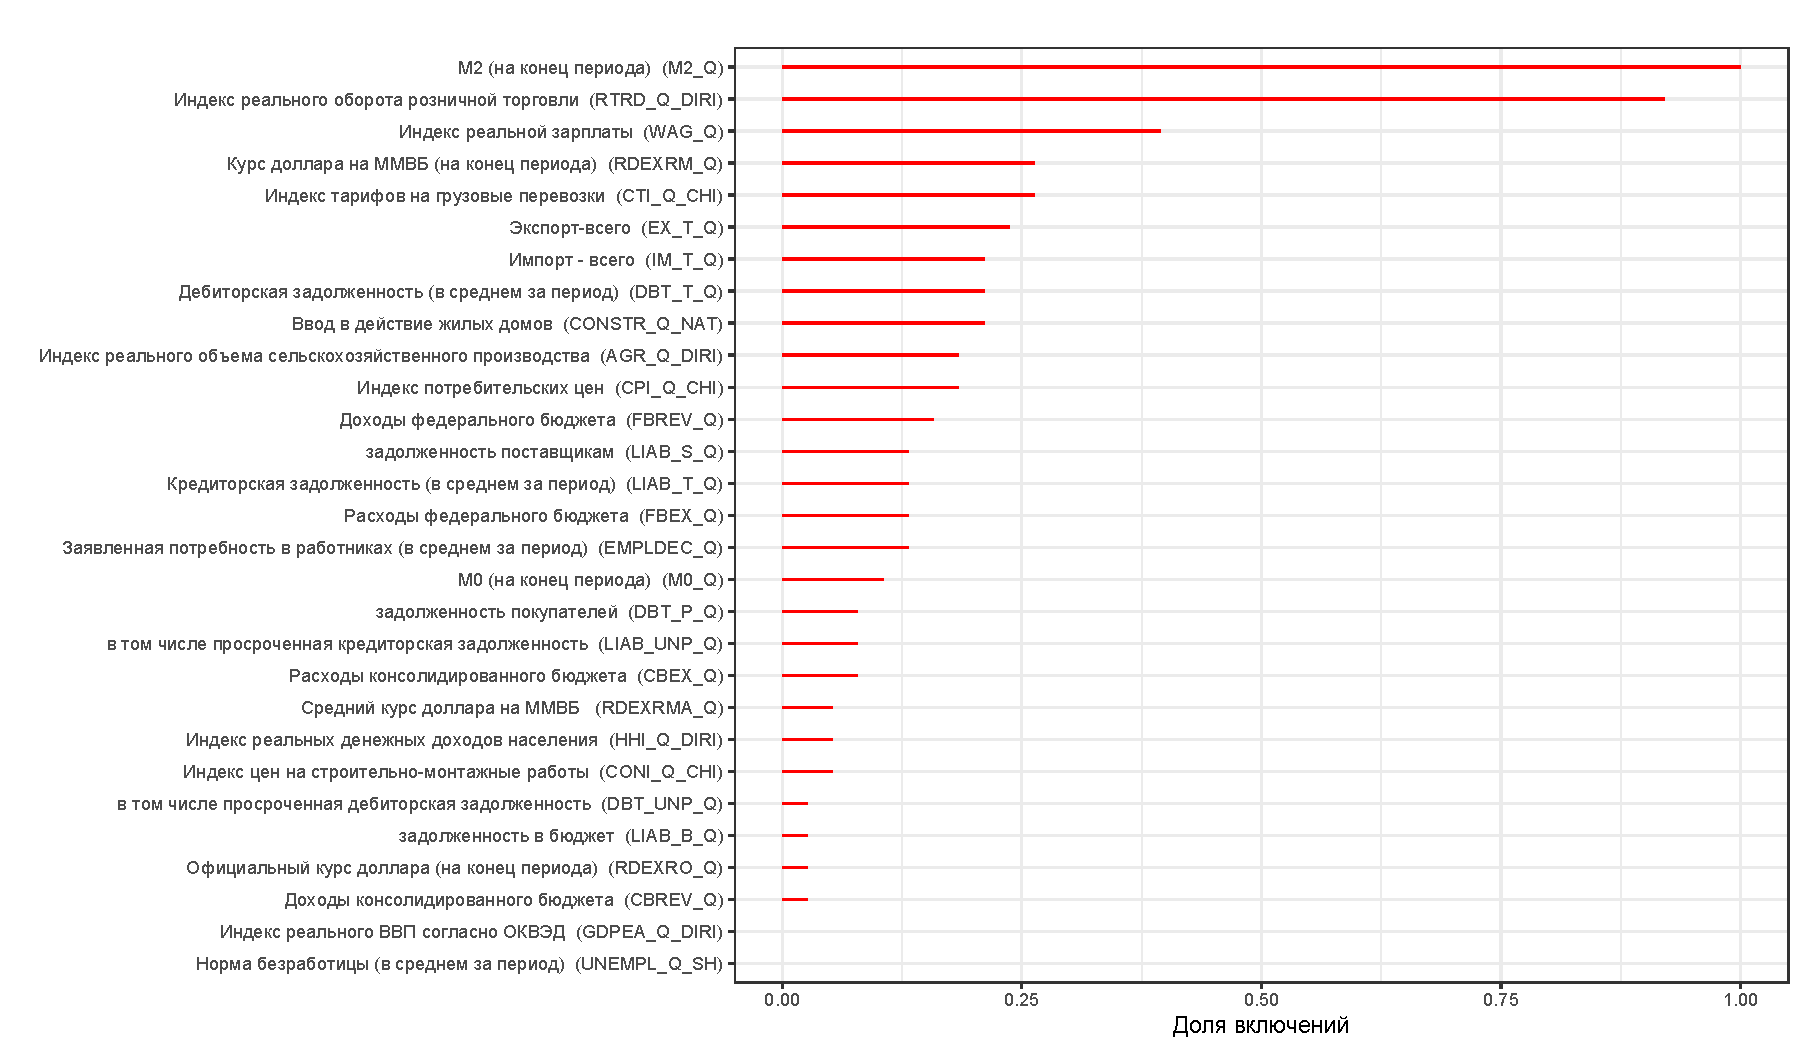
\includegraphics[width = \textwidth]{nzlollipop2.pdf}
    \caption{Включение переменных в модель LASSO}
    \label{fig:lp2}
\end{figure}

\begin{figure}[h]
    \centering
    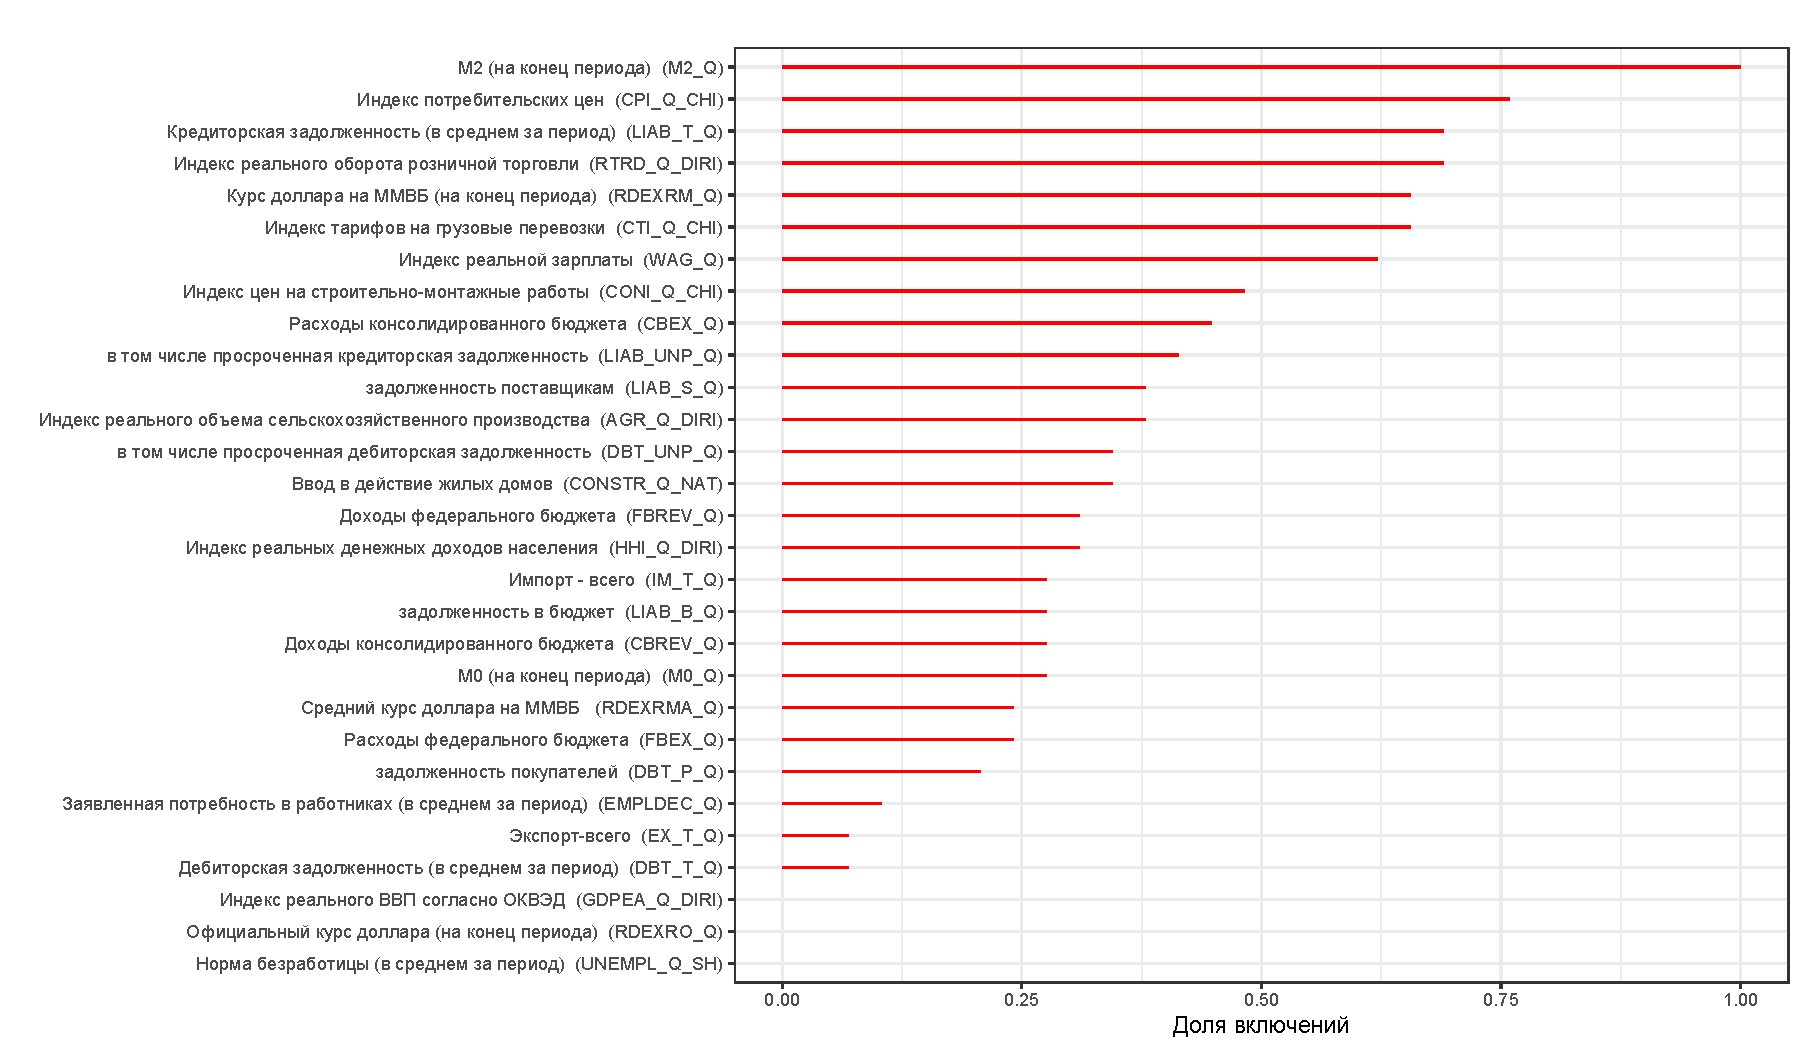
\includegraphics[width = \textwidth]{nzlollipop1.pdf}
    \caption{Включение переменных в модель Adaptive LASSO}
    \label{fig:lp1}
\end{figure}



Какие выводы можно сделать из этих двух диаграмм? Интересно, что обе модели выбирают в качестве объясняющей переменной денежный агрегат M2. Помимо этого можно отметить, что во многих спецификациях были важны индекс потребительских цен и кредиторская задолженность.



\section{Количество переменных и ошибки}

Главная опасность включения большого числа регрессоров в прогнозную модель --- это переобучение. Как говорилось ранее, методы регуляризации позволяют в какой-то мере избежать этой опасности. В неявном виде при использовании методов снижения размерности принимается предпосылка о том, что добавление большого количества регрессоров позволит улучшить качество модели. Но, может быть, для данных, используемых в данной работе это не справедливо? возможно, что те спецификации моделей, которые сильнее сокращали количество коэффициентов, показали лучшие результаты? В пользу этого предположения говорит и то, что модель регрессии гребня показала среди трех моделей с регуляризацией худшие результаты, а ее отличие от двух других моделей (LASSO и эластичной сети) как раз в том и состоит, что в ней невозможно полностью исключение переменных.

На рисунке \ref{fig:nzerror} можно видеть распределение ошибок в разных моделях с регуляризацией в зависимости от количества включённых переменных. В целом можно видеть отрицательную зависимость этих двух показателей для моделей, которые показывали наилучшее качество, и, значит, на данных, используемых в этой работе, включение переменных в модели с регуляризацией в среднем уменьшало ошибки (конечно, до какого-то предела --- как говорилось выше, в модели, не исключающей переменные, ошибки получились большими). Конечно, нельзя воспринимать это эмпирическое наблюдение как доказательство некоторых статистических закономерностей, т.к. он основан лишь на том ограниченном наборе данных, который использовался в данной работе.


\begin{figure}[h]
    \centering
    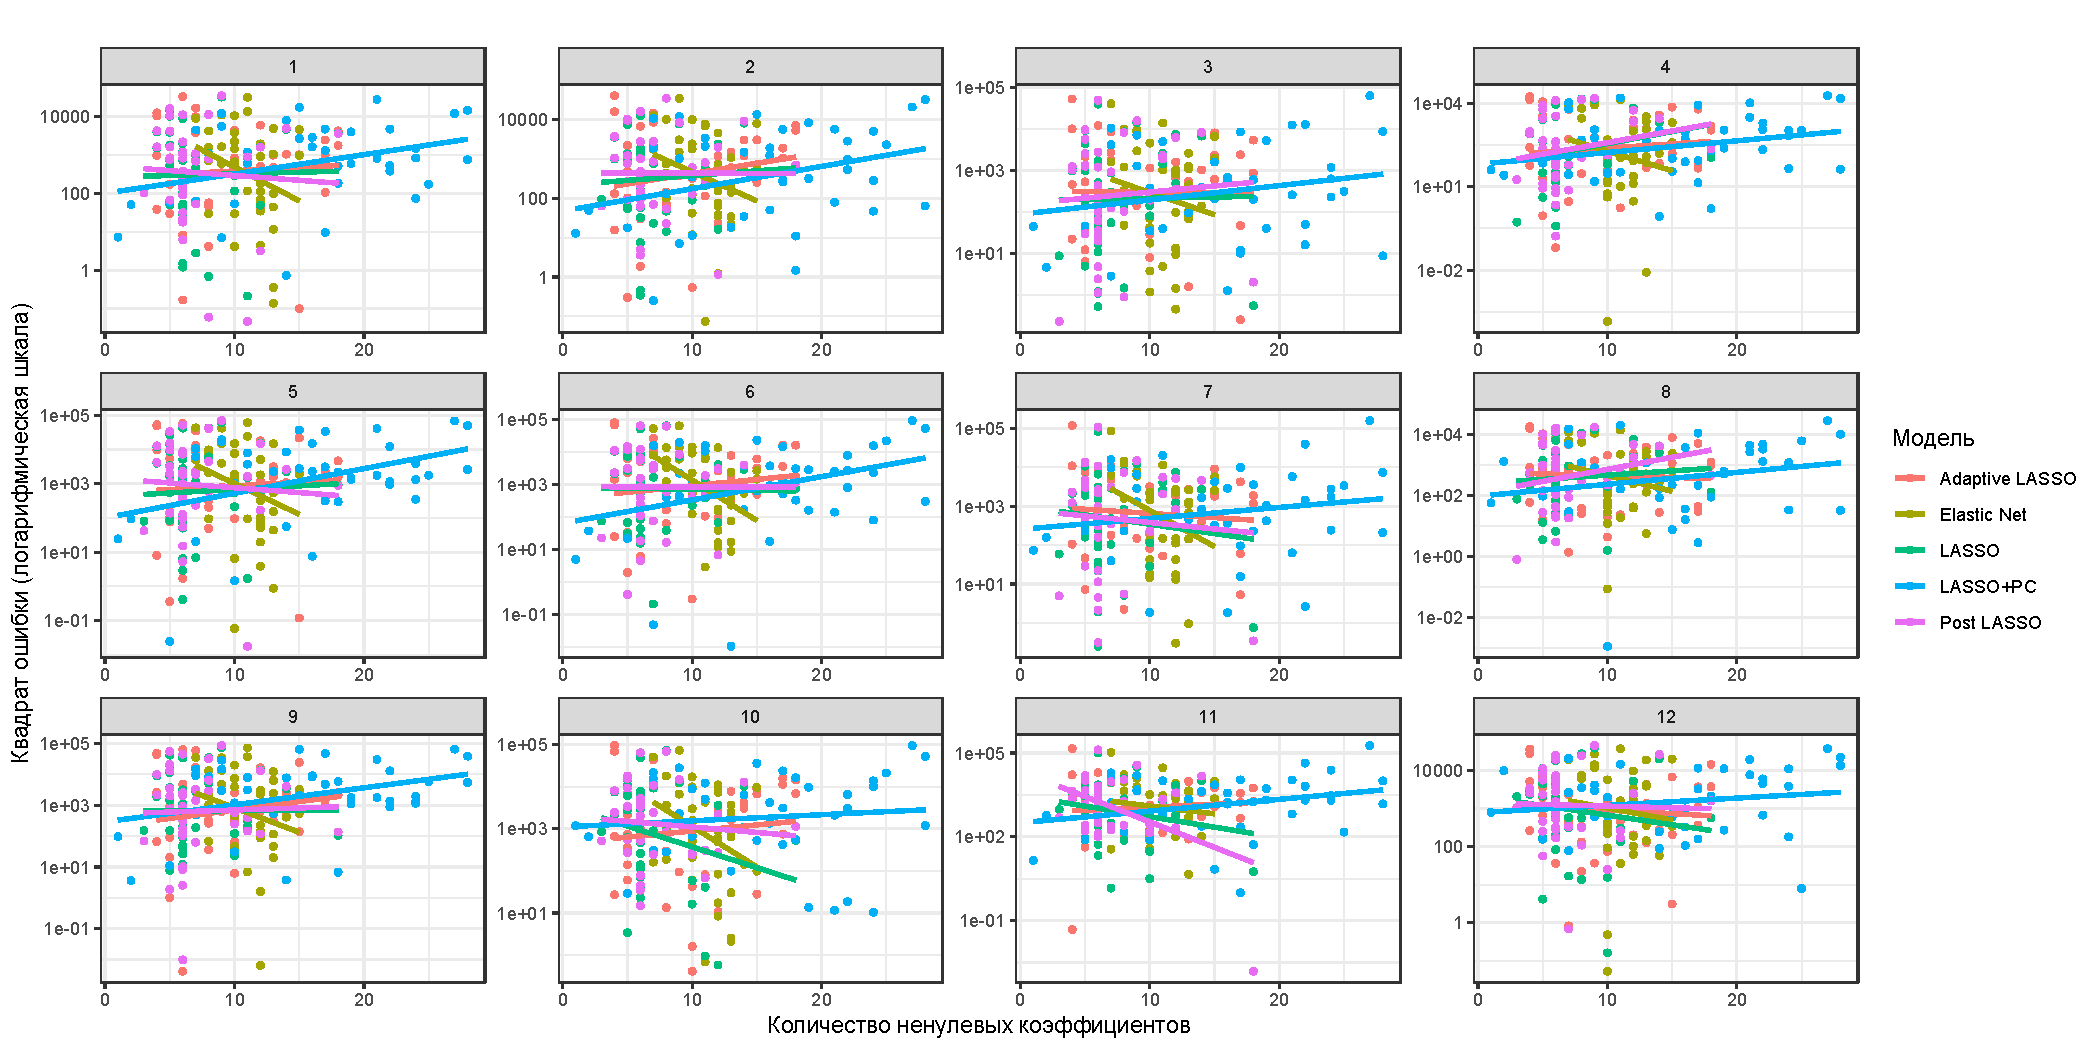
\includegraphics[width = \textwidth]{nonzeroerror.pdf}
    \caption{Распределение ошибок в зависимости от количества включённых переменных для моделей с регуляризацией}
    \label{fig:nzerror}
\end{figure}

Соображения, приведенные выше, не были бы полными, если бы не рассматривалось, в какие именно моменты времени спецификация тех или иных моделей приводила к определенному количеству коэффициентов. На рисунке \ref{fig:nztime} это показано. В целом можно отметить, что с течением времени у большинства моделей количество включённых коэффициентов колеблется вокруг одного уровня.

\begin{figure}[h]
    \centering
    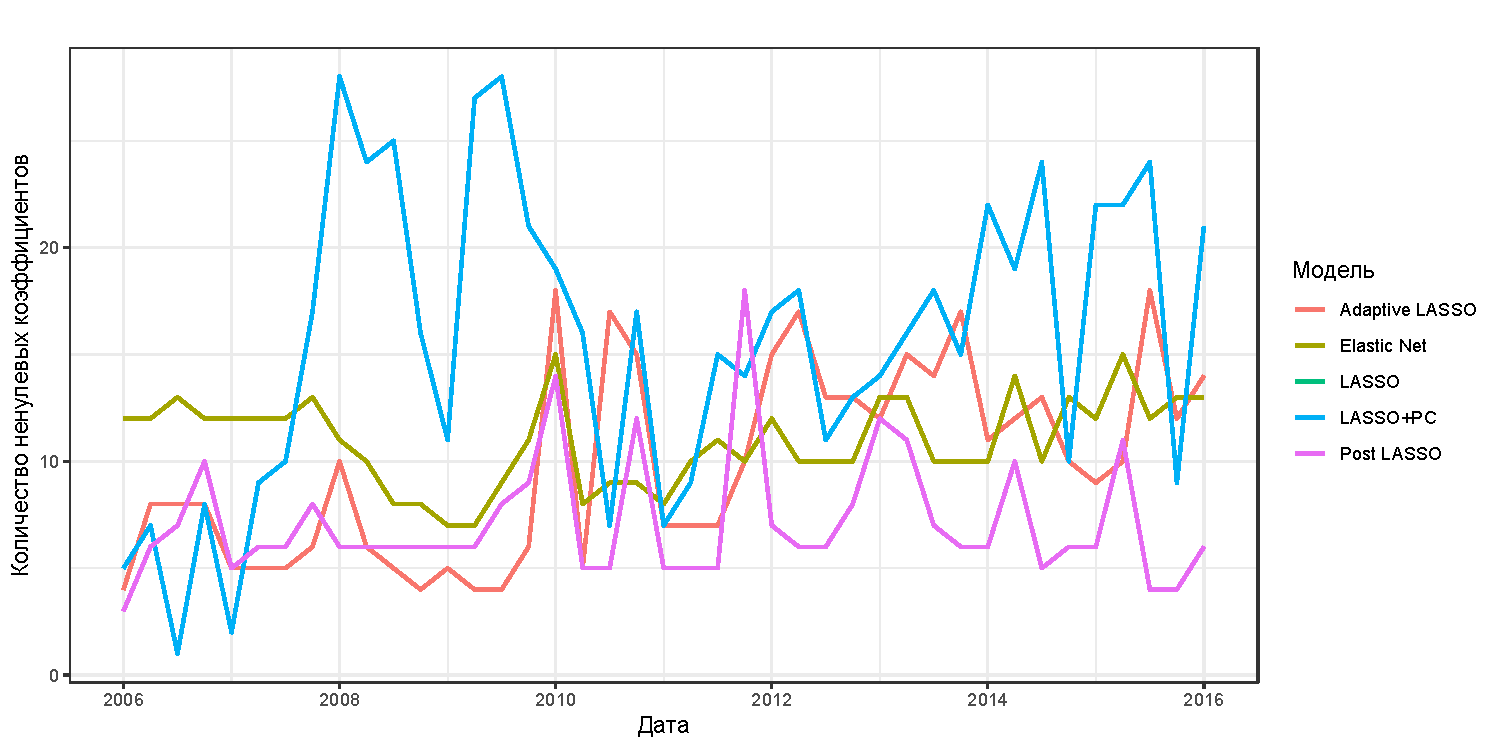
\includegraphics[width = \textwidth]{nonzerotime.pdf}
    \caption{Количество ненулевых коэффициентов для моделей с регуляризацией}
    \label{fig:nztime}
\end{figure}

\chapter*{Заключение} \label{ch:final}\addcontentsline{toc}{chapter}{\protect\numberline{Заключение}}

В результате оценки и прогнозирования инвестиций в России на основе макроэкономических данных высокой размерности с помощью методов снижения размерности были получены хорошие относительно базовой модели традиционной акселераторной результаты для методов LASSO, Adaptive LASSO, бустинга, пик-плато и случайного леса (для разных горизонтов прогнозирования). В целом это согласуется с результатами аналогичного анализа в работе \cite{baybuza2018inflation}, где исследовались методы машинного обучения для прогнозирования месячной инфляция в России. Однако в данной работе модель бустинга всегда показывала лучшие результаты. Видимо, это можно объяснить, во-первых, тем, что при использовании месячных данных естественным образом возникает больше наблюдений, а во-вторых, тем, что месячные данные больше подвержены случайным флуктуациям, и в результате модель бустинга, многократно пересматривающаяся в ходе обучения, даёт более консервативные прогнозы, чем сильнее подверженная переобучению модель LASSO или, тем более, модель регрессии гребня.

Можно неудовлевторительно заметить, что ни одна из используемых моделей не смогла в достаточной мере предсказать как минимум за год падение уровня выпуска и инвестиций при кризисах 2007--2008 гг. и 2014--2015 гг.

Модель бустинга показала нормальность остатков прогнозов для горизонта прогноза, большего чем 5 кварталов, что увеличивает мотивацию использовать е для практического применения в виде прогноозирования инвестиций в России на срок до 3 лет вперед. 

В ходе работы также были обнаружены некоторые любопытные зависимости между макроэкономическими рядами, которые необходимо исследовать подробнее. 
Эмпирически на данных, используемых в работе, условно подтвердилось предположение о росте качества моделей при включении в них новых переменных.

\newpage
\label{ch:final}\addcontentsline{toc}{chapter}{\protect\numberline{Список литературы}}


\printbibliography

\newpage

\begin{appendices}
\chapter[]{Список используемых переменных}\label{app:list}



\begin{table}[ht]
\centering
\begin{tabular}{l}
  \hline
Название переменной \\ 
  \hline
Норма безработицы (в среднем за период)  (UNEMPL\_Q\_SH) \\ 
  Заявленная потребность в работниках (в среднем за период)  (EMPLDEC\_Q) \\ 
  Ввод в действие жилых домов  (CONSTR\_Q\_NAT) \\ 
  Индекс реальной зарплаты  (WAG\_Q) \\ 
  Индекс потребительских цен  (CPI\_Q\_CHI) \\ 
  Индекс цен на строительно-монтажные работы  (CONI\_Q\_CHI) \\ 
  Индекс тарифов на грузовые перевозки  (CTI\_Q\_CHI) \\ 
  Индекс реального объема сельскохозяйственного производства  (AGR\_Q\_DIRI) \\ 
  Индекс реального оборота розничной торговли  (RTRD\_Q\_DIRI) \\ 
  Индекс реальных денежных доходов населения  (HHI\_Q\_DIRI) \\ 
  М0 (на конец периода)  (M0\_Q) \\ 
  М2 (на конец периода)  (M2\_Q) \\ 
  Доходы консолидированного бюджета  (CBREV\_Q) \\ 
  Расходы консолидированного бюджета  (CBEX\_Q) \\ 
  Доходы федерального бюджета  (FBREV\_Q) \\ 
  Расходы федерального бюджета  (FBEX\_Q) \\ 
  Официальный курс доллара (на конец периода)  (RDEXRO\_Q) \\ 
  Курс доллара на ММВБ (на конец периода)  (RDEXRM\_Q) \\ 
  Средний курс доллара на ММВБ   (RDEXRMA\_Q) \\ 
  Кредиторская задолженность (в среднем за период)  (LIAB\_T\_Q) \\ 
  в том числе просроченная кредиторская задолженность  (LIAB\_UNP\_Q) \\ 
  задолженность поставщикам  (LIAB\_S\_Q) \\ 
  задолженность в бюджет  (LIAB\_B\_Q) \\ 
  Дебиторская задолженность (в среднем за период)  (DBT\_T\_Q) \\ 
  в том числе просроченная дебиторская задолженность  (DBT\_UNP\_Q) \\ 
  задолженность покупателей  (DBT\_P\_Q) \\ 
  Экспорт-всего  (EX\_T\_Q) \\ 
  Импорт - всего  (IM\_T\_Q) \\ 
  Индекс реального ВВП согласно ОКВЭД  (GDPEA\_Q\_DIRI) \\ 
   \hline
\end{tabular}
\end{table}
\newpage


\chapter[]{Дополнительные метрики качества}\label{app:score}

\begin{table}[ht]
\centering
\caption{MAE для горизонта прогнозирования от 1 до 6 кварталов относительно акселераторной модели}
\begin{tabular}{lrrrrrr}
  \hline
Модель & 1 & 2 & 3 & 4 & 5 & 6 \\ 
  \hline
Adaptive LASSO & 0.80 & 0.92 & 1.01 & 1.06 & 1.04 & 1.08 \\ 
  Boosting & 2.00 & 1.45 & 1.16 & 1.07 & 0.90 & 0.83 \\ 
  Elastic Net & 0.80 & 0.91 & 0.97 & 1.06 & 1.05 & 1.05 \\ 
  LASSO & 0.85 & 0.93 & 0.99 & 1.08 & 1.06 & 1.06 \\ 
  LASSO+PC & 0.91 & 0.89 & 1.02 & 1.17 & 1.15 & 1.16 \\ 
  LASSO+VAR & 0.97 & 1.01 & 1.04 & 1.06 & 0.98 & 0.90 \\ 
  Post LASSO & 0.78 & 0.91 & 0.99 & 1.08 & 1.06 & 1.10 \\ 
  Random Forest & 0.86 & 0.87 & 0.83 & 0.99 & 0.92 & 0.90 \\ 
  Ridge & 0.79 & 0.89 & 0.95 & 1.08 & 1.06 & 1.05 \\ 
  Spike and Slab & 0.79 & 0.91 & 0.99 & 1.07 & 1.07 & 1.06 \\ 
   \hline
\end{tabular}
\end{table}


\begin{table}[ht]
\centering
\caption{MAE для горизонта прогнозирования от 7 до 12 кварталов относительно акселераторной модели}
\begin{tabular}{lrrrrrr}
  \hline
Модель & 7 & 8 & 9 & 10 & 11 & 12 \\ 
  \hline
Adaptive LASSO & 1.11 & 1.10 & 1.11 & 1.17 & 1.21 & 1.19 \\ 
  Boosting & 0.80 & 0.78 & 0.72 & 0.69 & 0.69 & 0.68 \\ 
  Elastic Net & 1.06 & 1.07 & 1.07 & 1.08 & 1.14 & 1.12 \\ 
  LASSO & 1.06 & 1.07 & 1.07 & 1.07 & 1.13 & 1.10 \\ 
  LASSO+PC & 1.19 & 1.27 & 1.30 & 1.29 & 1.34 & 1.38 \\ 
  LASSO+VAR & 0.96 & 1.08 & 1.07 & 1.08 & 1.08 & 1.05 \\ 
  Post LASSO & 1.11 & 1.12 & 1.13 & 1.16 & 1.22 & 1.19 \\ 
  Random Forest & 0.93 & 1.01 & 0.94 & 0.93 & 0.98 & 1.04 \\ 
  Ridge & 1.07 & 1.09 & 1.08 & 1.08 & 1.15 & 1.15 \\ 
  Spike and Slab & 1.08 & 1.07 & 1.09 & 1.08 & 1.14 & 1.11 \\ 
   \hline
\end{tabular}
\end{table}


\begin{table}[ht]
\centering
\caption{$R^2$ для горизонта прогнозирования от 1 до 6 кварталов}
\begin{tabular}{lrrrrrr}
  \hline
Модель & 1 & 2 & 3 & 4 & 5 & 6 \\ 
  \hline
Adaptive LASSO & 0.76 & 0.34 & -0.26 & -0.77 & -1.49 & -1.99 \\ 
  Boosting & -0.25 & -0.30 & -0.36 & -0.40 & -0.43 & -0.46 \\ 
  Elastic Net & 0.75 & 0.33 & -0.19 & -0.67 & -1.28 & -1.62 \\ 
  LASSO & 0.74 & 0.33 & -0.20 & -0.67 & -1.28 & -1.61 \\ 
  LASSO+PC & 0.74 & 0.39 & -0.28 & -1.07 & -2.21 & -2.81 \\ 
  LASSO+VAR & 0.60 & 0.23 & -0.22 & -0.41 & -0.58 & -0.61 \\ 
  Post LASSO & 0.78 & 0.34 & -0.25 & -0.78 & -1.48 & -1.92 \\ 
  Random Forest & 0.70 & 0.39 & 0.00 & -0.43 & -0.76 & -0.98 \\ 
  Ridge & 0.75 & 0.35 & -0.21 & -0.71 & -1.31 & -1.63 \\ 
  Spike and Slab & 0.77 & 0.38 & -0.18 & -0.68 & -1.37 & -1.74 \\ 
   \hline
\end{tabular}
\end{table}

\begin{table}[ht]
\centering
\caption{$R^2$ для горизонта прогнозирования от 7 до 12 кварталов}
\begin{tabular}{lrrrrrr}
  \hline
Модель & 7 & 8 & 9 & 10 & 11 & 12 \\ 
  \hline
Adaptive LASSO & -2.45 & -2.47 & -3.30 & -4.23 & -5.04 & -4.99 \\ 
  Boosting & -0.50 & -0.53 & -0.63 & -0.72 & -0.75 & -0.75 \\ 
  Elastic Net & -1.92 & -1.93 & -2.55 & -3.14 & -3.58 & -3.55 \\ 
  LASSO & -1.88 & -1.89 & -2.53 & -3.08 & -3.48 & -3.41 \\ 
  LASSO+PC & -3.72 & -4.35 & -5.92 & -7.40 & -8.99 & -10.66 \\ 
  LASSO+VAR & -0.93 & -1.55 & -2.59 & -4.00 & -5.10 & -5.64 \\ 
  Post LASSO & -2.32 & -2.37 & -3.18 & -3.95 & -4.63 & -4.69 \\ 
  Random Forest & -1.19 & -1.37 & -1.54 & -1.86 & -2.03 & -2.20 \\ 
  Ridge & -1.99 & -2.01 & -2.57 & -3.17 & -3.65 & -3.63 \\ 
  Spike and Slab & -2.13 & -2.14 & -2.84 & -3.48 & -3.98 & -3.95 \\ 
   \hline
\end{tabular}
\end{table}


\end{appendices}
\end{document}